% Chapter 7

\chapter{Methodology} % Write in your own chapter title
\label{Chapter7}
\lhead{Chapter 7. \emph{Methodology}}

\section{Artificial Dataset}

The dataset, named a colour detector, is generated artificially. Each image has three labels to represent colours, $red$, $green$ and $blue$. If an image is a red hue only, it has a label for $red$ while the label values of $green$ and $blue$ are negative. The representation of colour combination follows colour wheels. If an image has a hue close to $purple$, it has positive labels for $red$ and $blue$, and negative label for $green$, and so on.
\graphicspath{ {./Figures/} }
\begin{figure}[!htb]
\centering
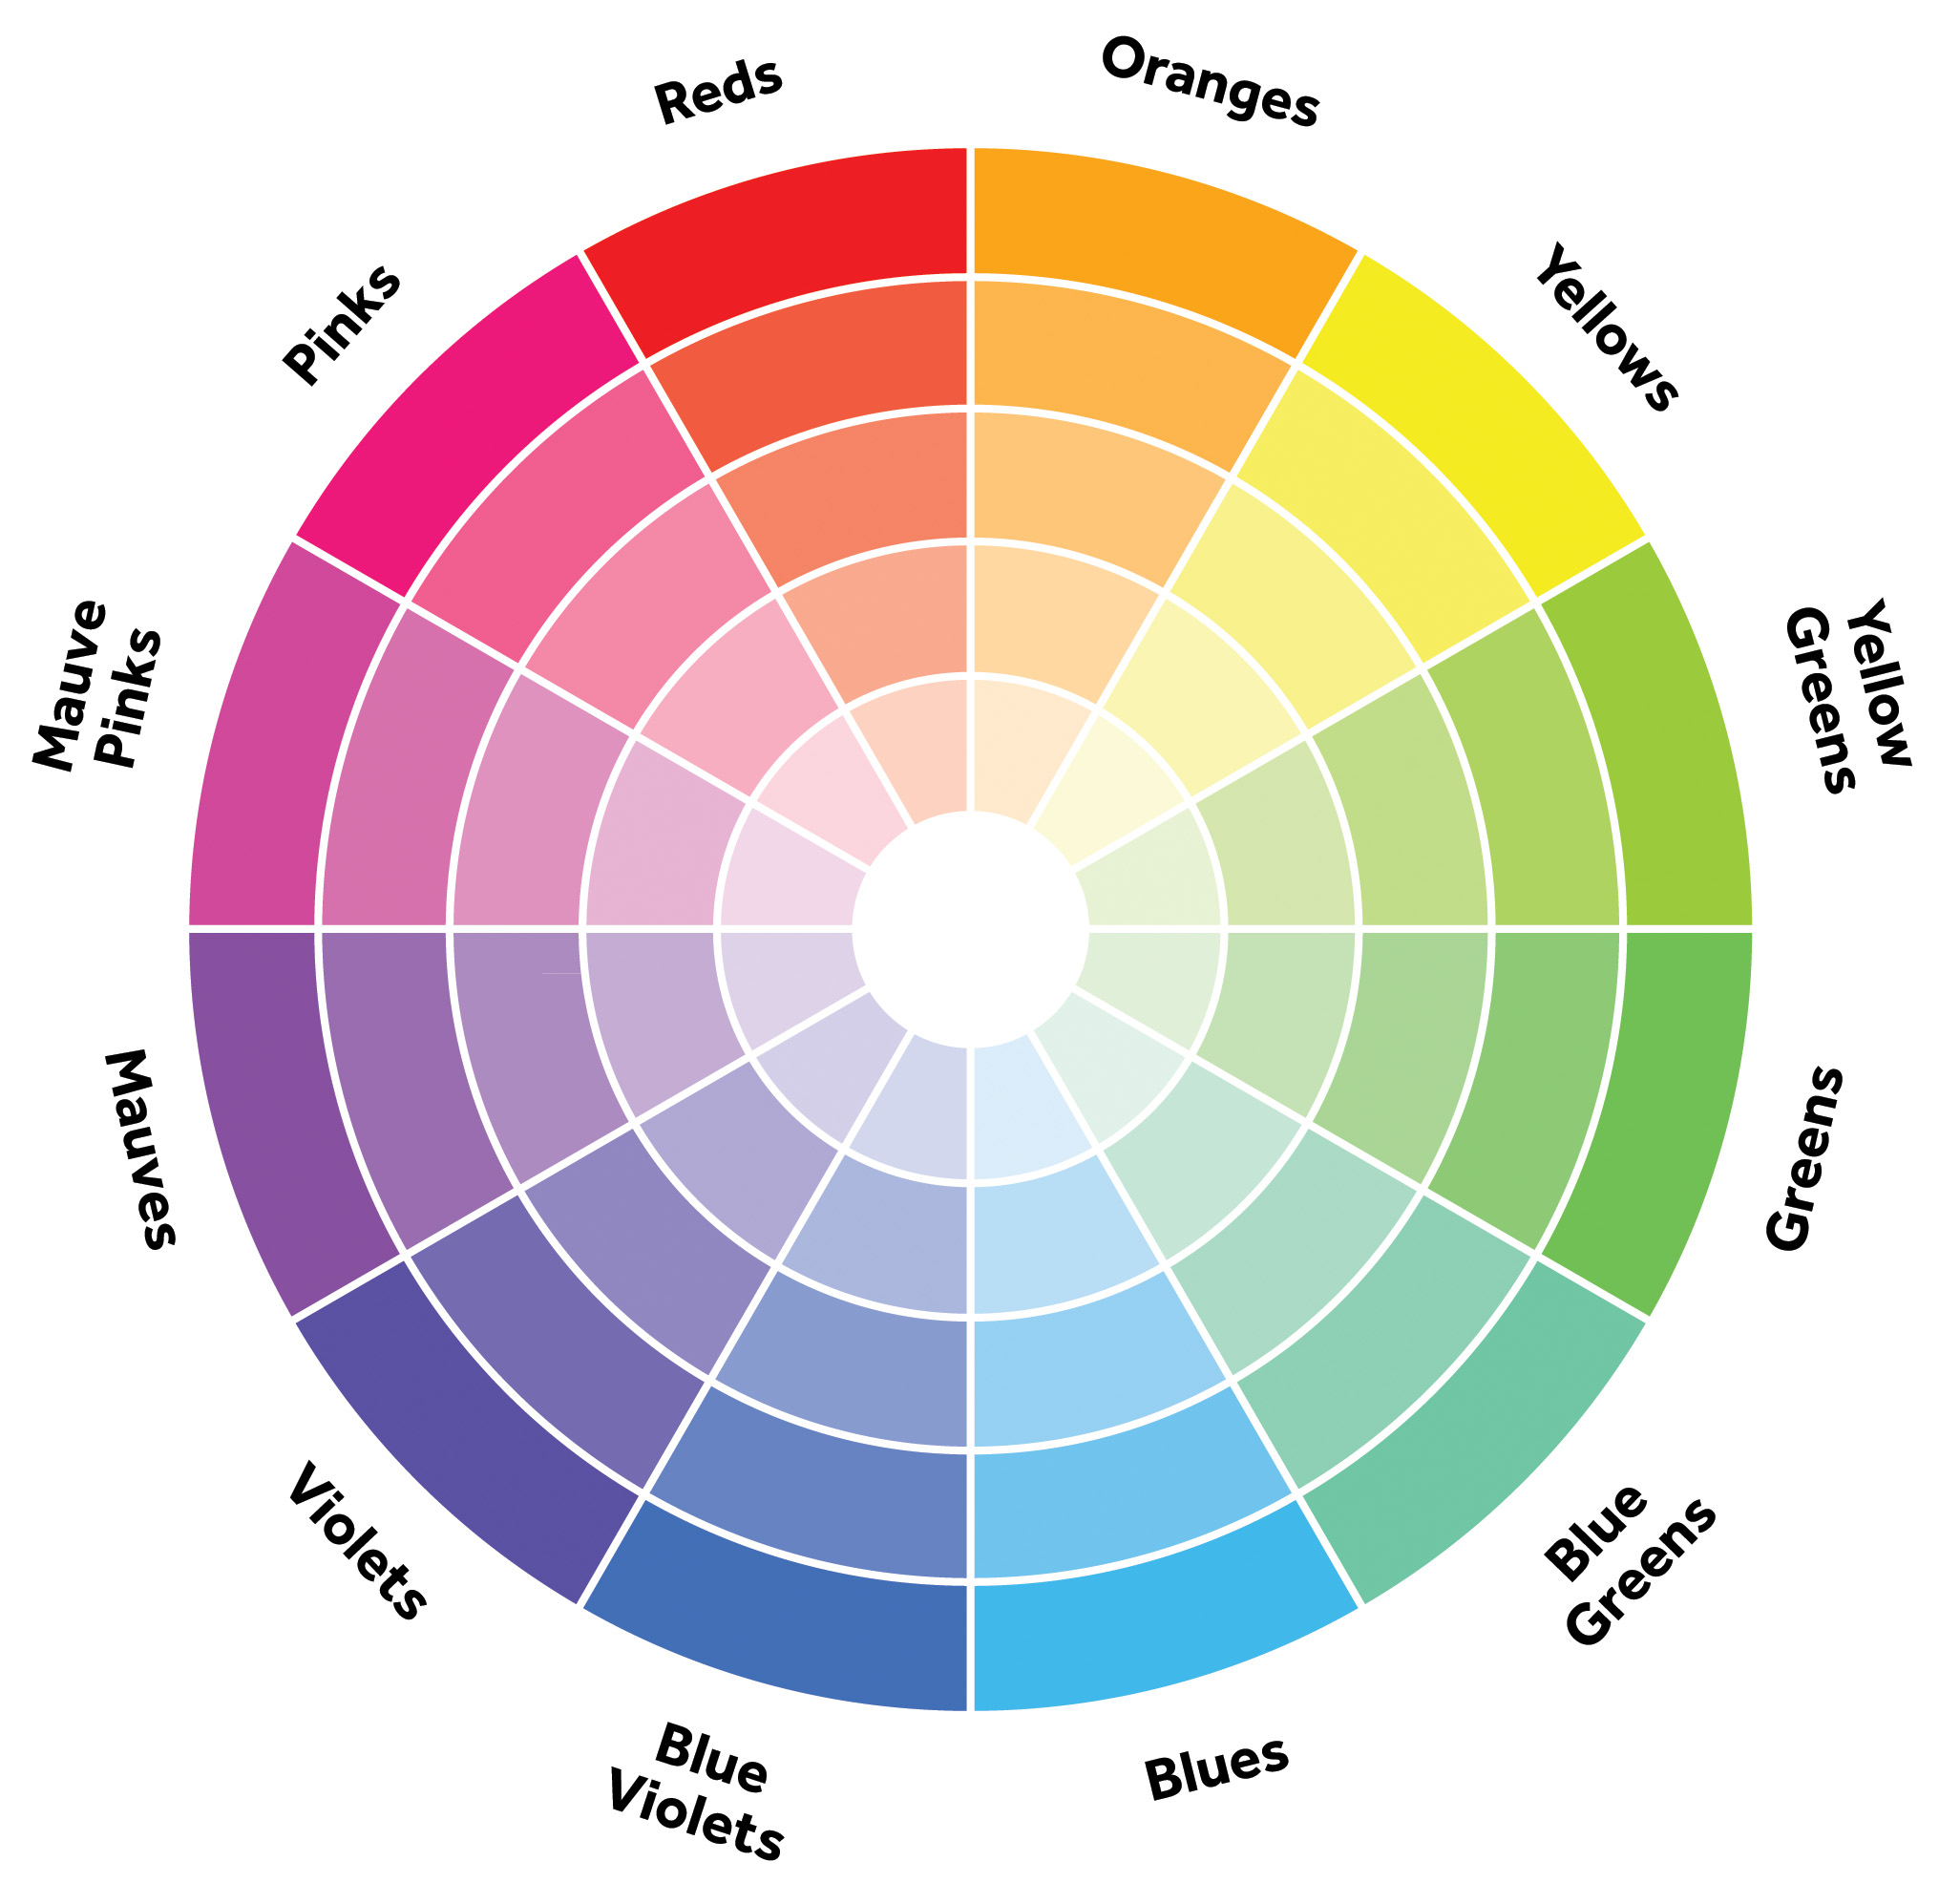
\includegraphics[scale=0.1]{color_wheel.jpg}
\caption{\label{fig:ColorWheel}Colour Wheel Diagram}
\end{figure}

For each sample $x_{i}$, it owns 3 labels ${y_{0},y_{1},y_{2}},  y_{j} \in \{-1,1\}$ which represent $red$, $green$ and $blue$ respectively.

\subsection{Generating images}

The RGB and HSV coordinate systems represent a geometric shape in colour space. The distance among colours contains little meaning. However, corresponding distance makes some intuitive sense and enable conversion possible between RGB coordinates and HSV coordinates.

The dataset consists of images with size $16x16$, so each image has $256$ pixels. To generate an image, I generate a random floating point number $h$ in the range $[0.0, 1.0)$ and use it as value for a hue via formulation.
\begin{equation}\label{eq:FormulationHue}
H = h + r * 0.4 - 0.2 (r \in [0.0,1.0))
\end{equation}
Where $r$ is another random floating point number. We generate 2 random floating point numbers for Saturation(S) and Value(V) values. The HSV values are converted to the RGB values and timed $255$ for each pixel. Following that, an image with $256$ pixels is generated. Because a RGB image is converted to a HSV image, the label values are based on the previous value $h$.

\graphicspath{ {./Figures/RGBhist/} }
\begin{figure}[!htb]
\centering     %%% not \center
\subfigure[Label:1 -1 1]{
\includegraphics[width=0.2\textwidth]{0}}
\subfigure{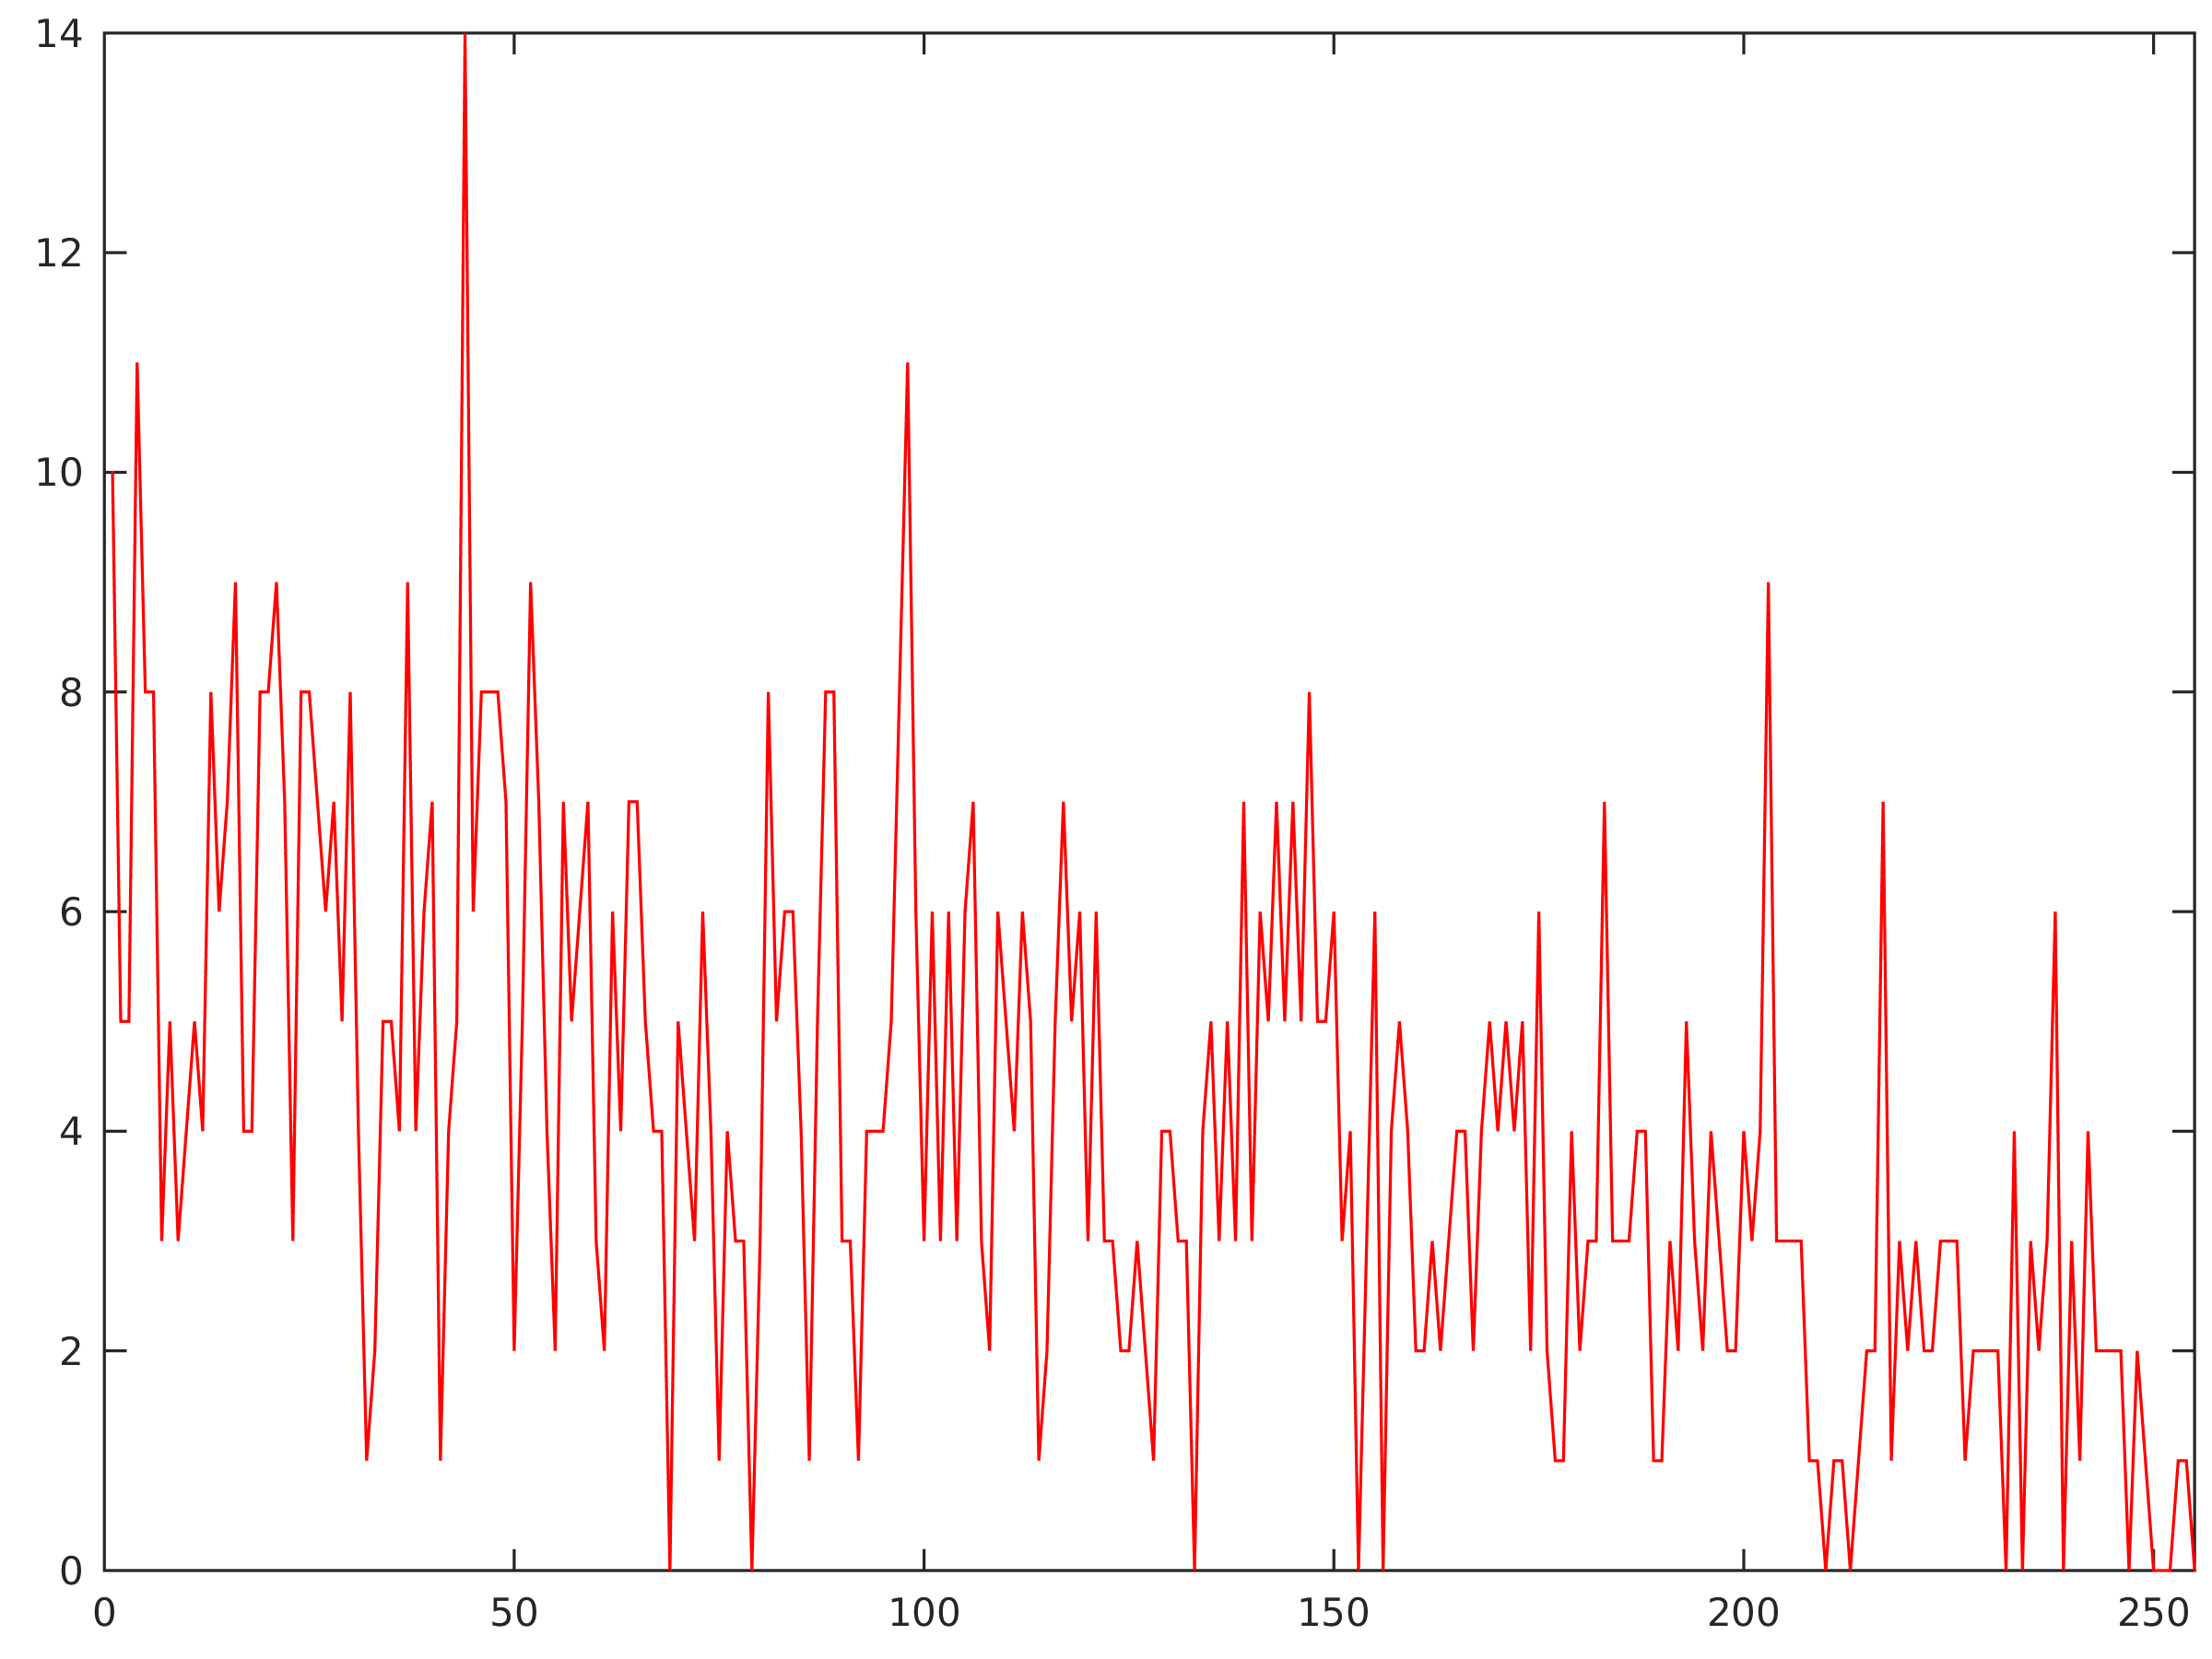
\includegraphics[width=0.25\textwidth]{0r}}
\subfigure{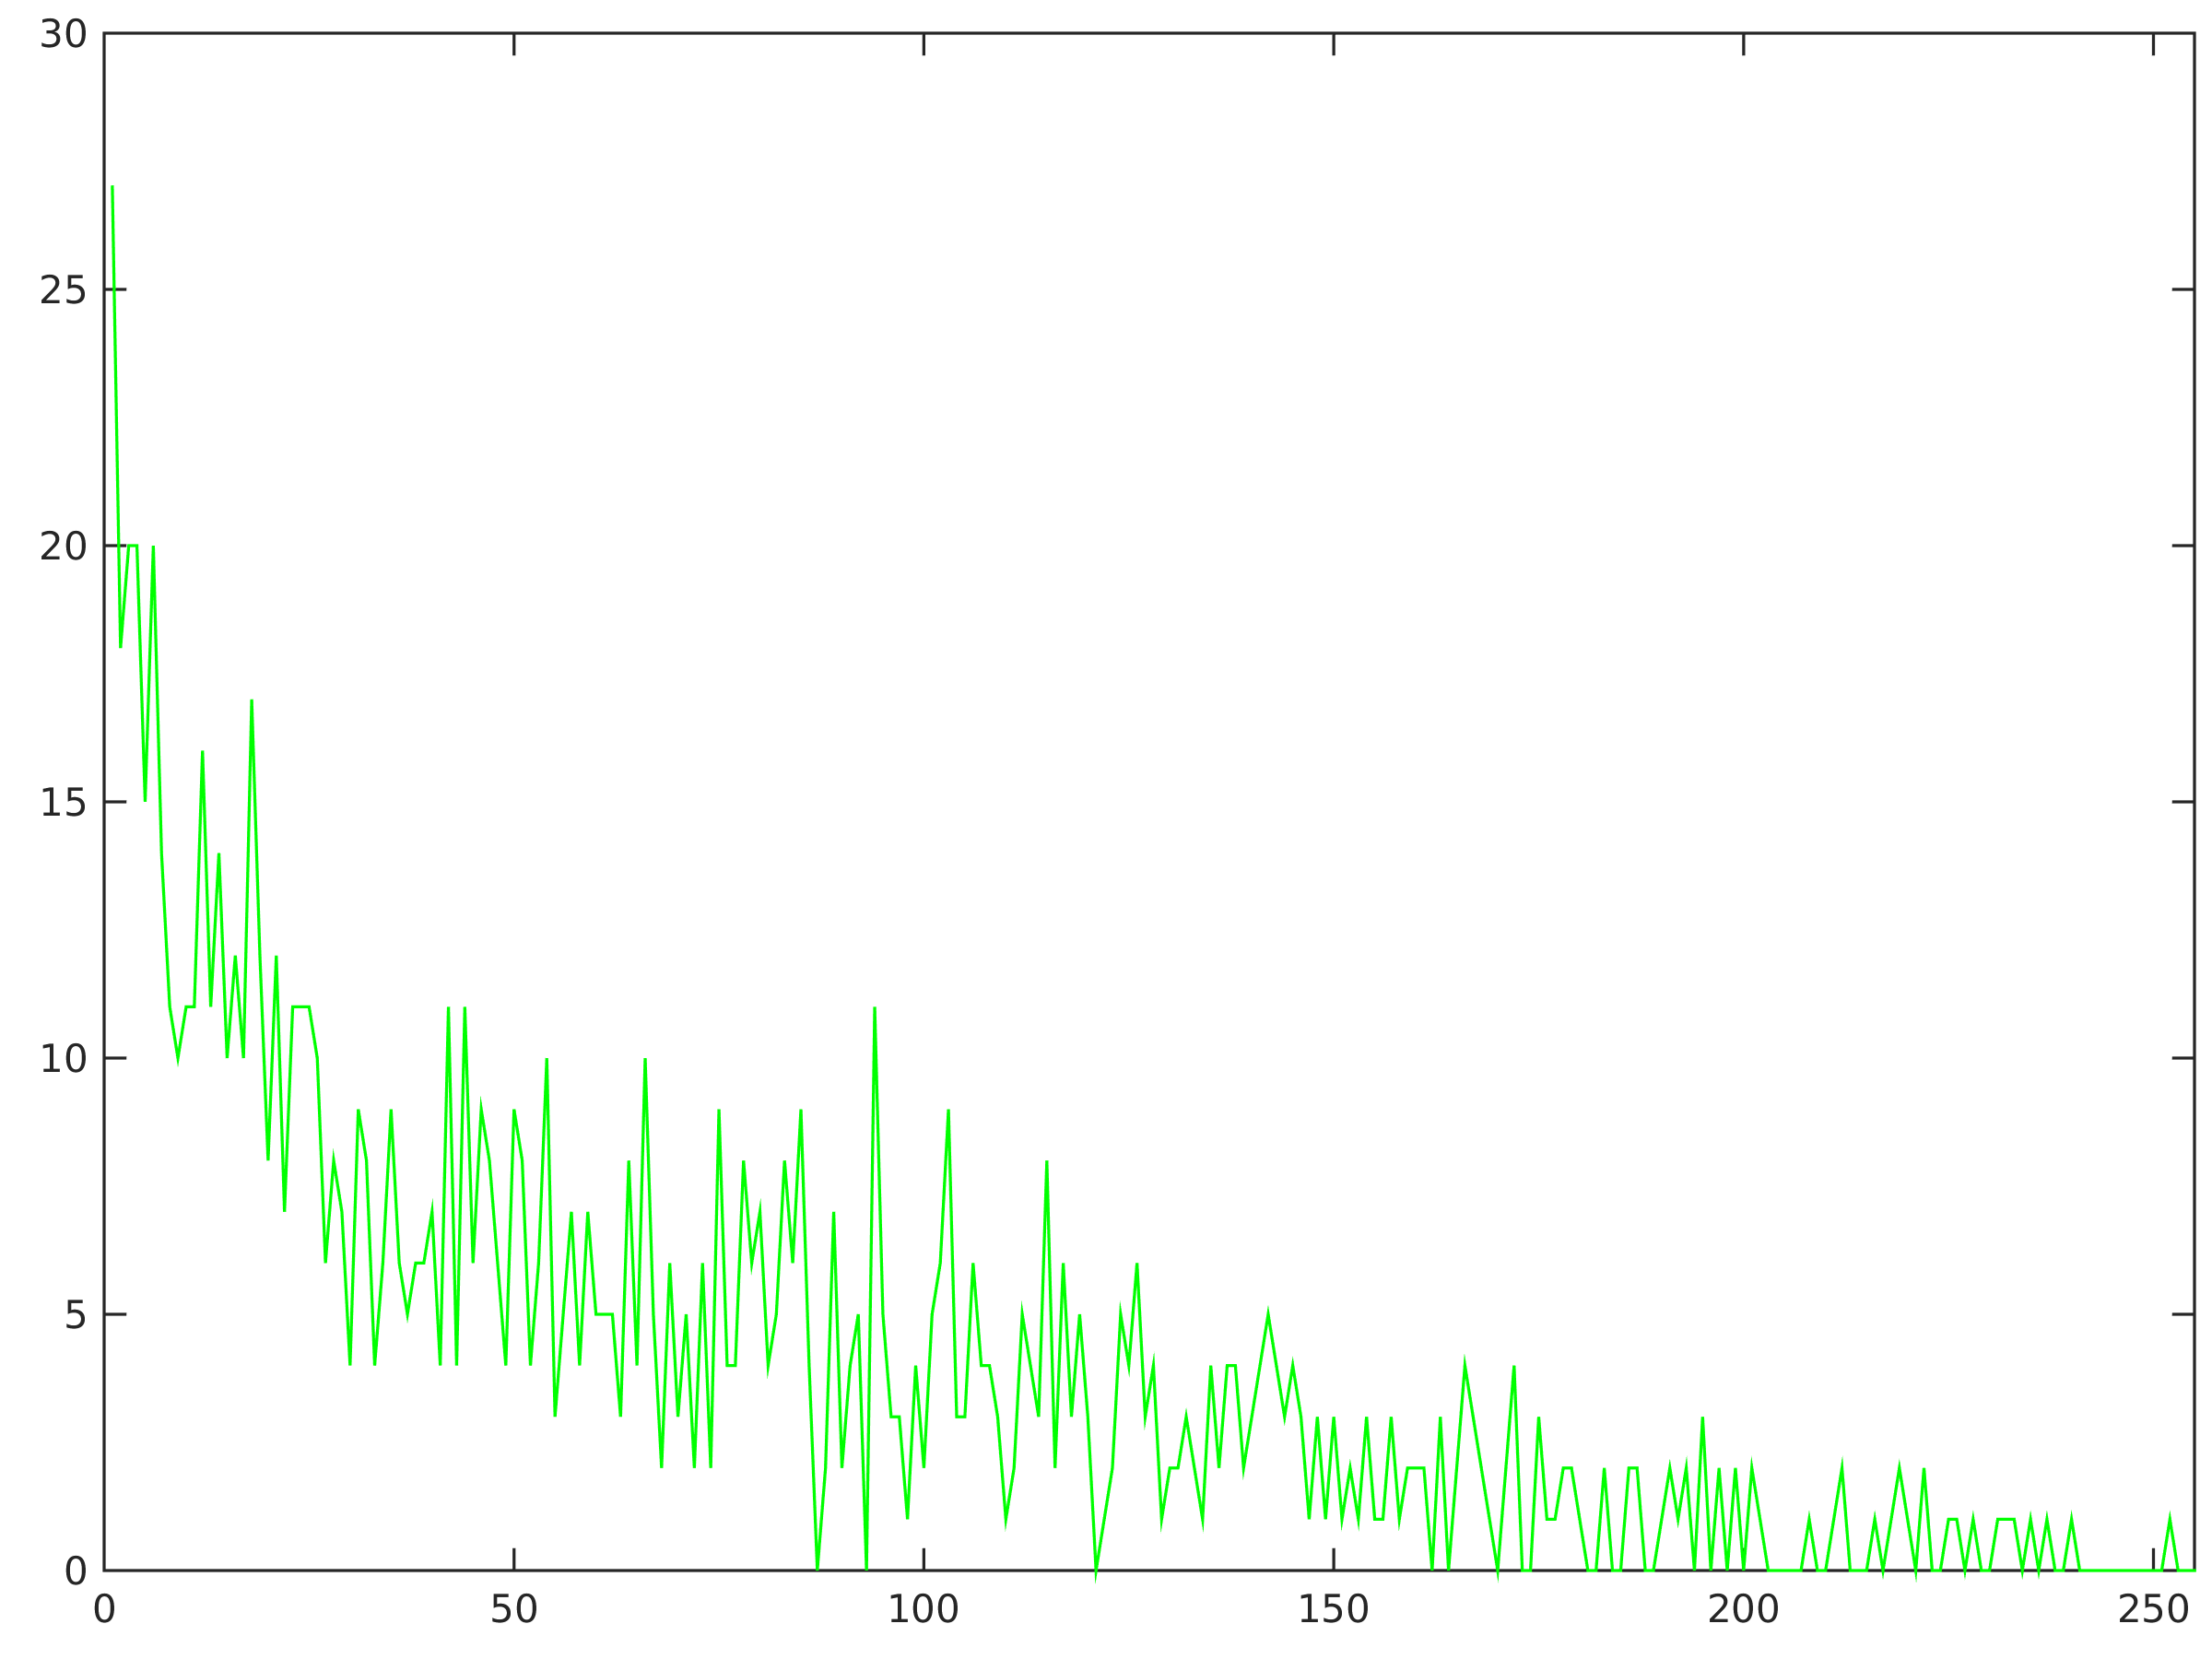
\includegraphics[width=0.25\textwidth]{0g}}
\subfigure{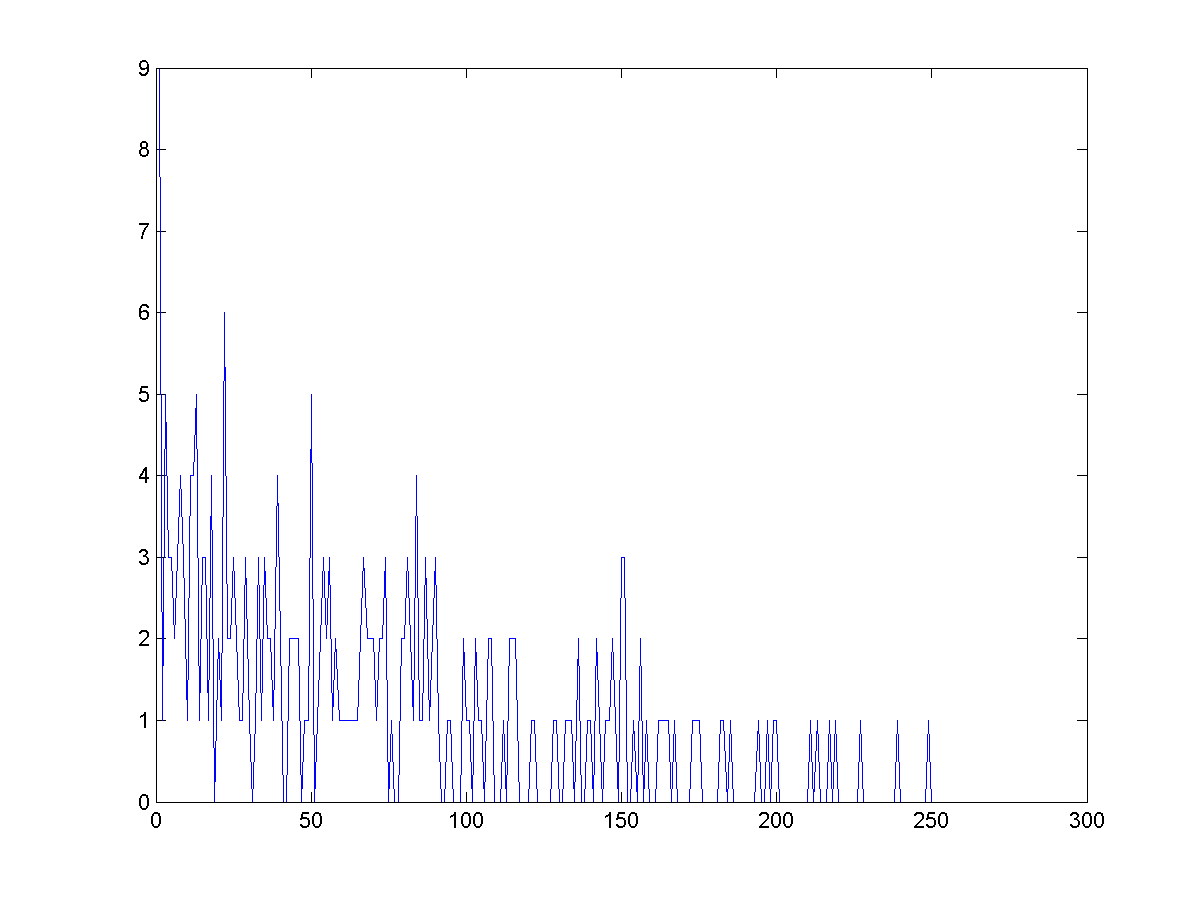
\includegraphics[width=0.25\textwidth]{0b}}
\subfigure[Label:1 1 -1]{
\includegraphics[width=0.2\textwidth]{1}}
\subfigure{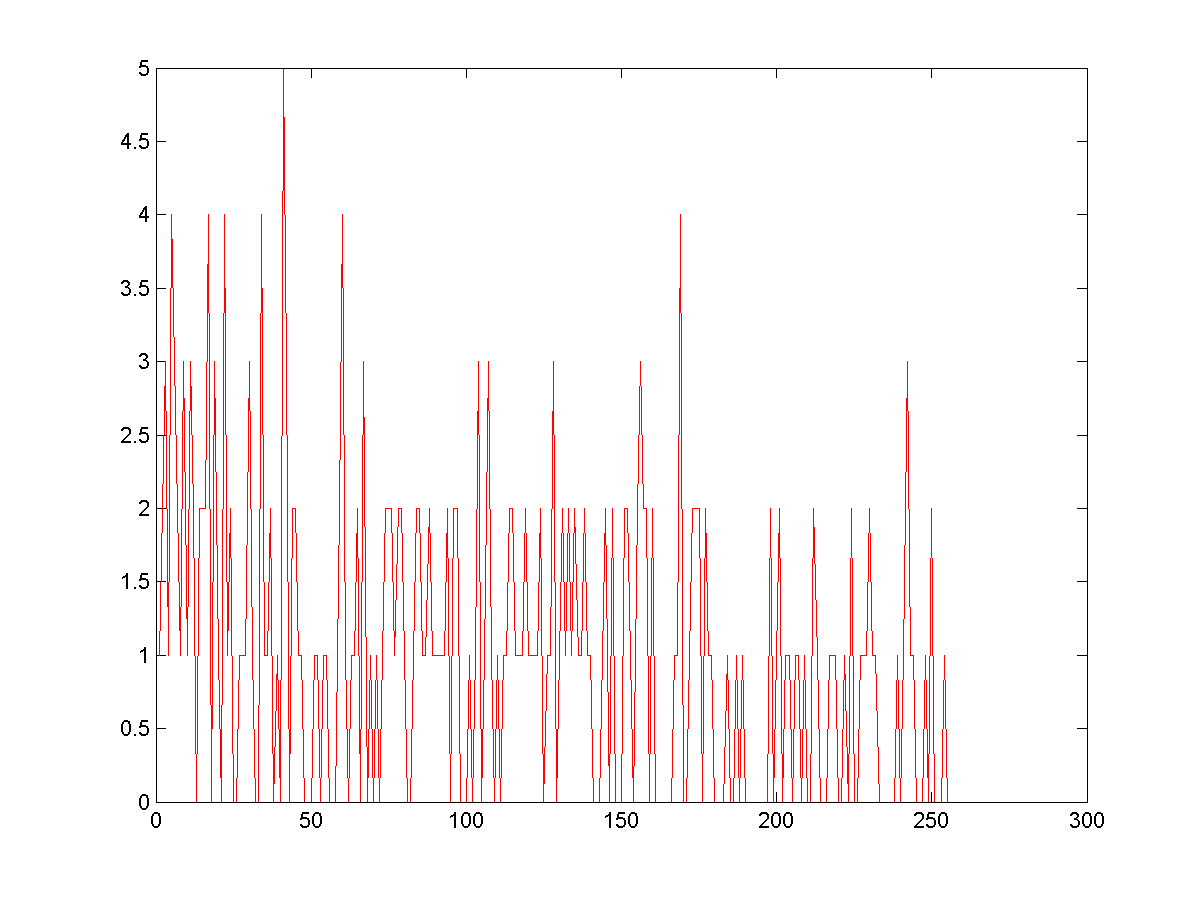
\includegraphics[width=0.25\textwidth]{1r}}
\subfigure{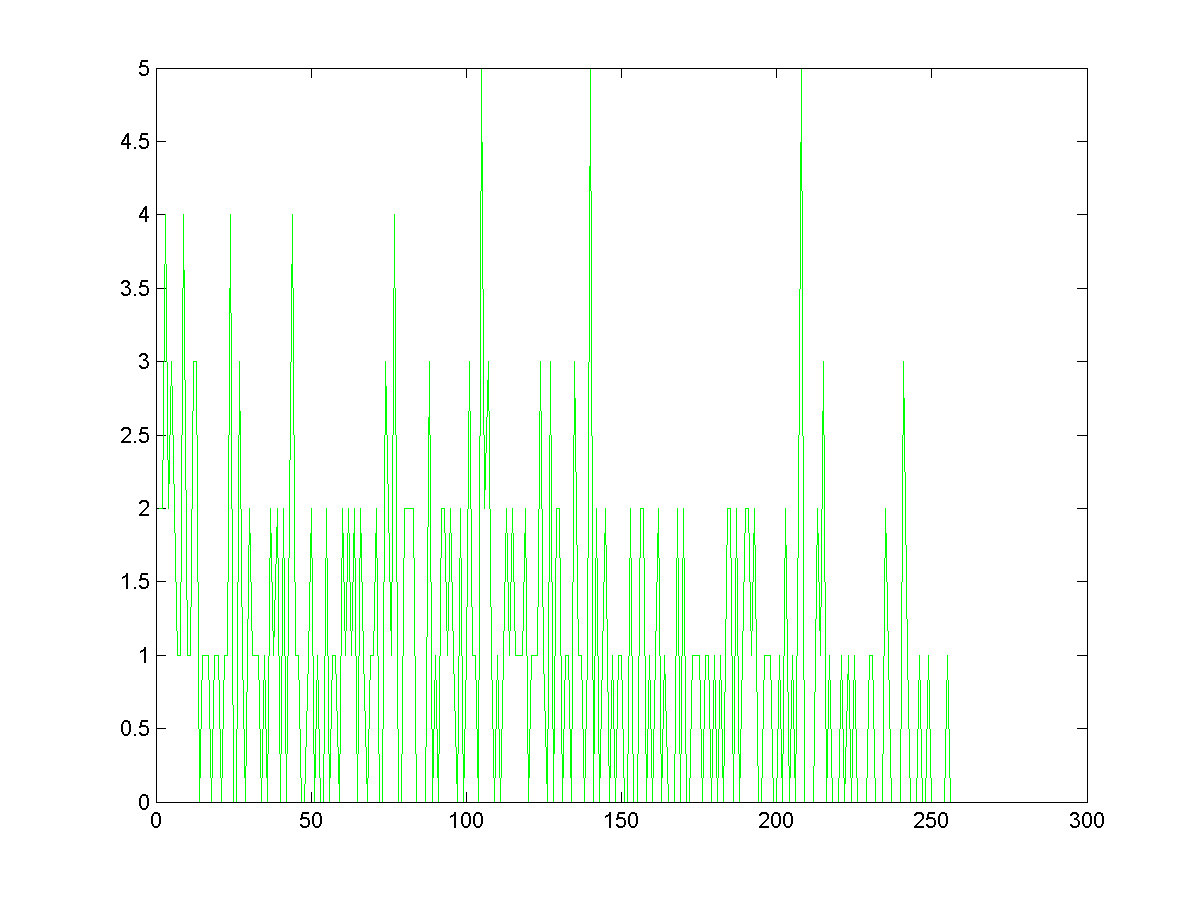
\includegraphics[width=0.25\textwidth]{1g}}
\subfigure{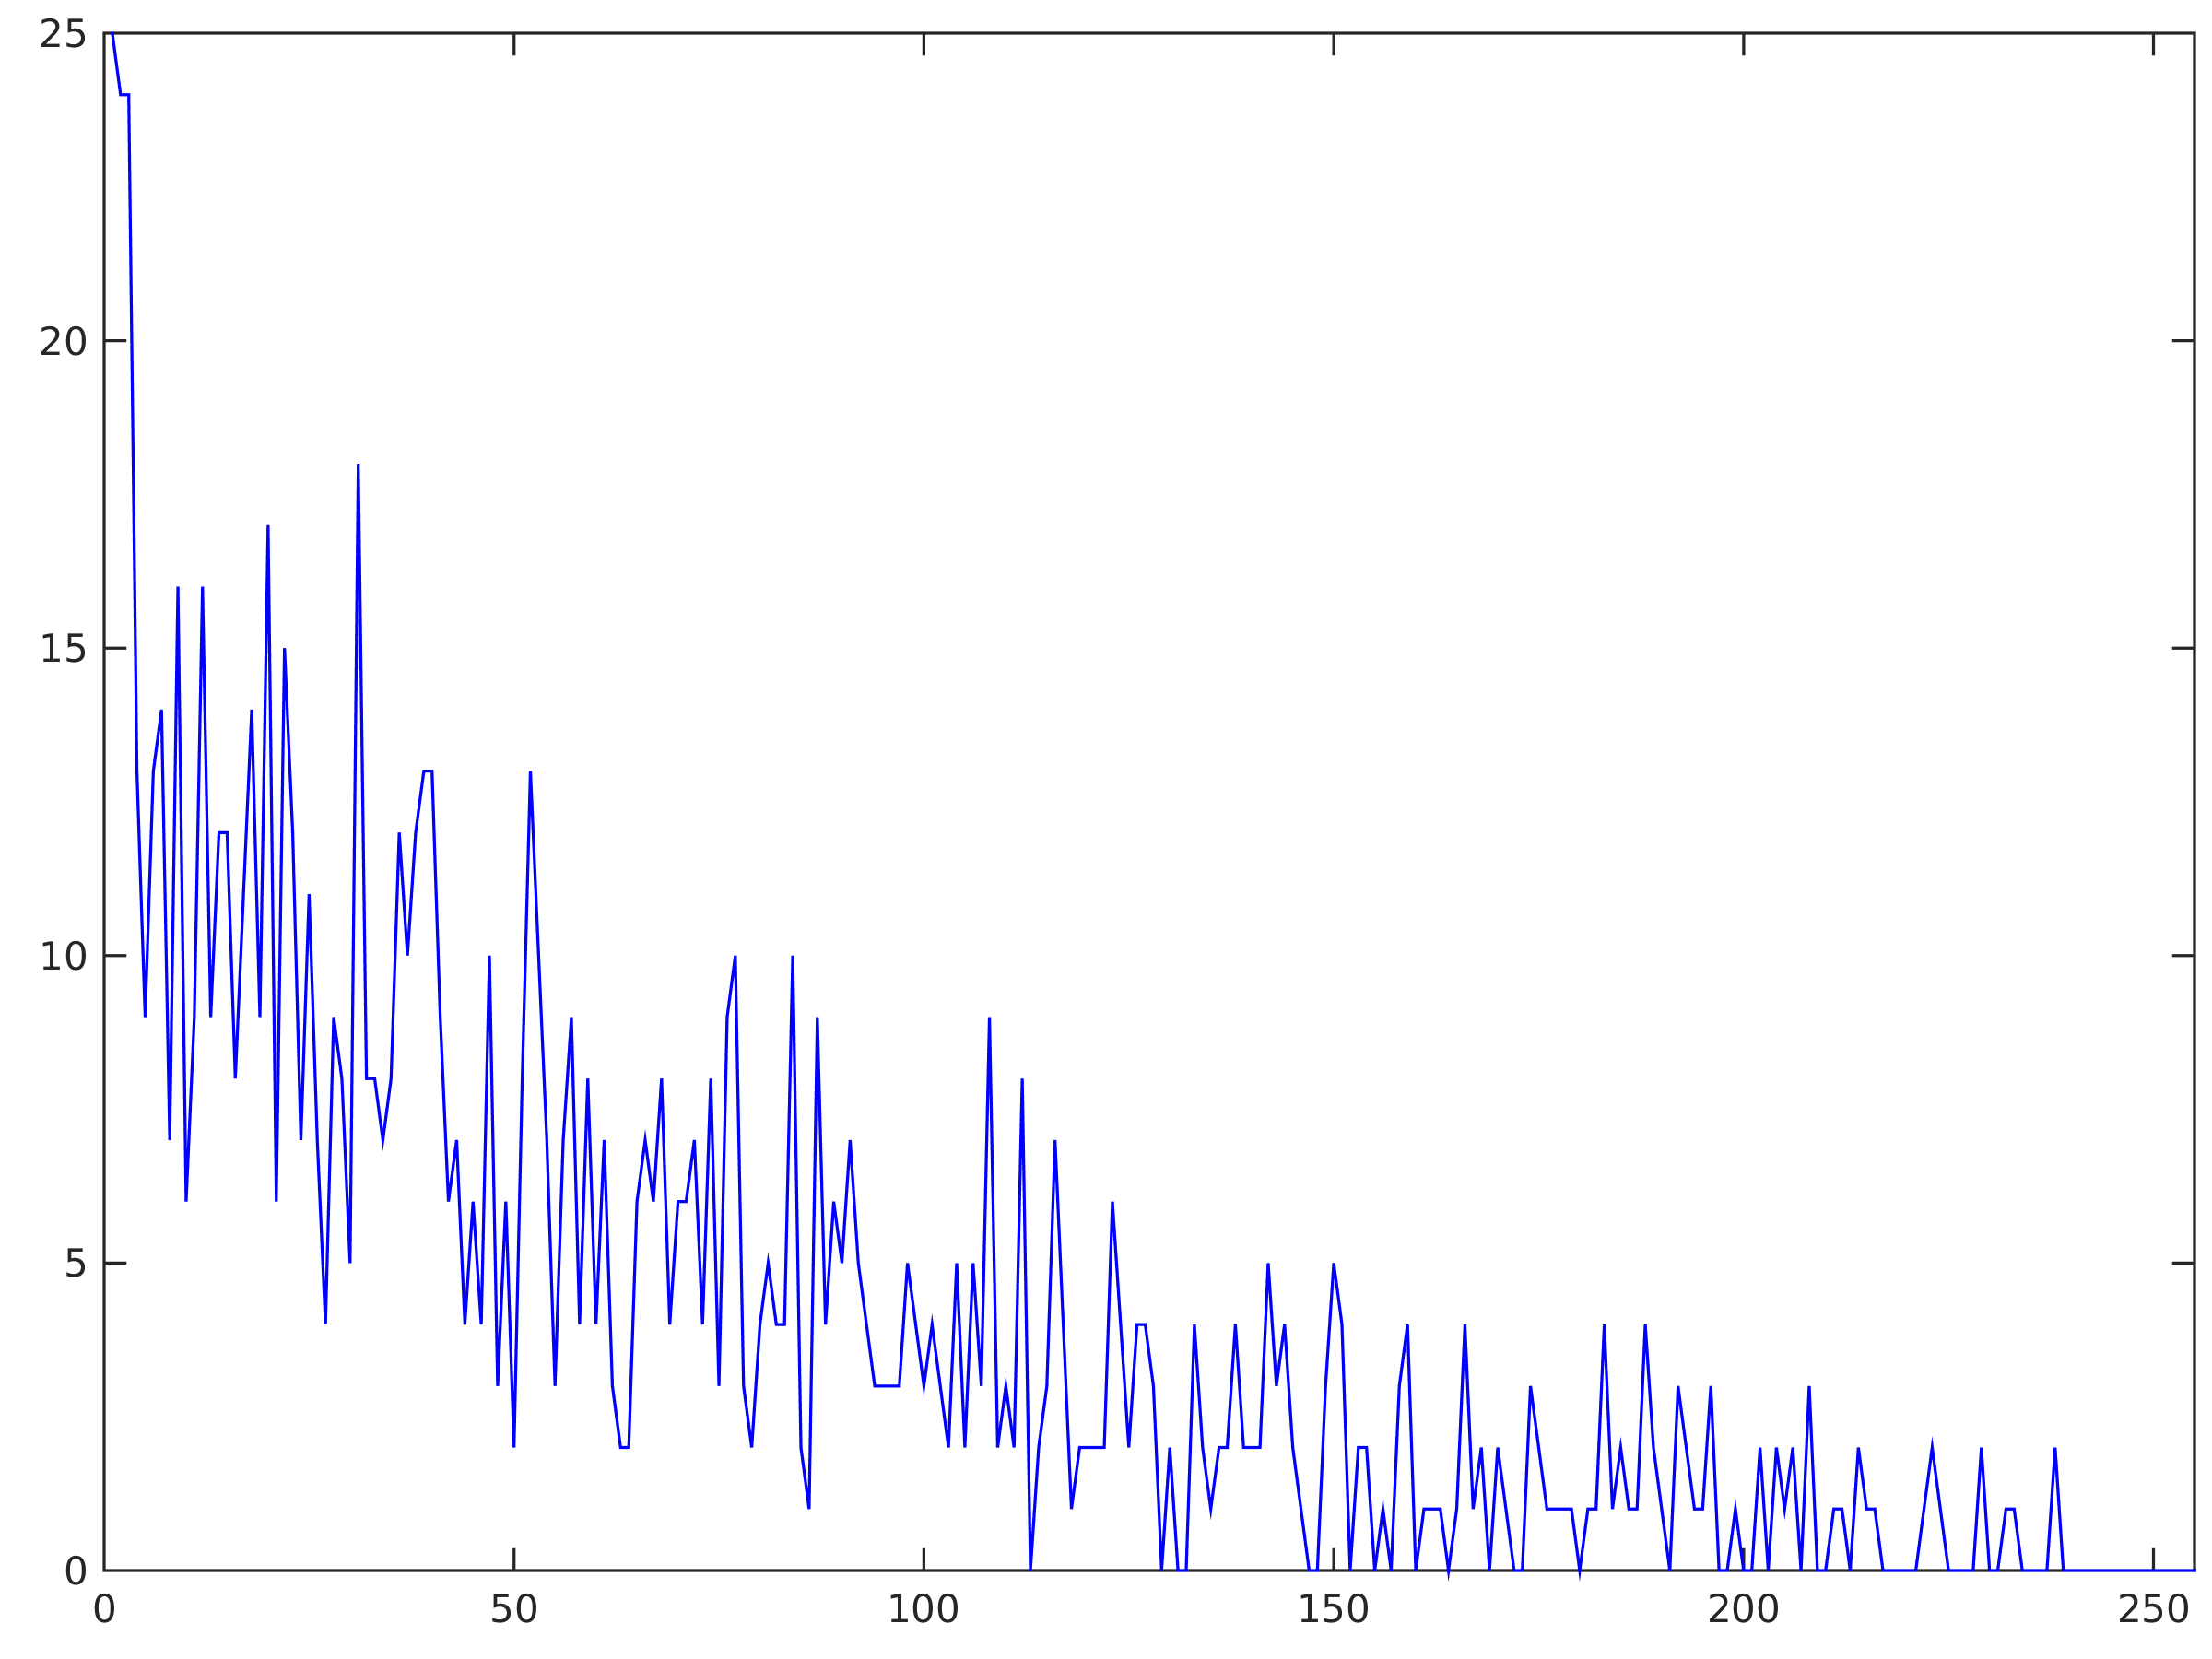
\includegraphics[width=0.25\textwidth]{1b}}
\subfigure[Label:-1 1 -1]{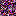
\includegraphics[width=0.2\textwidth]{2}}
\subfigure{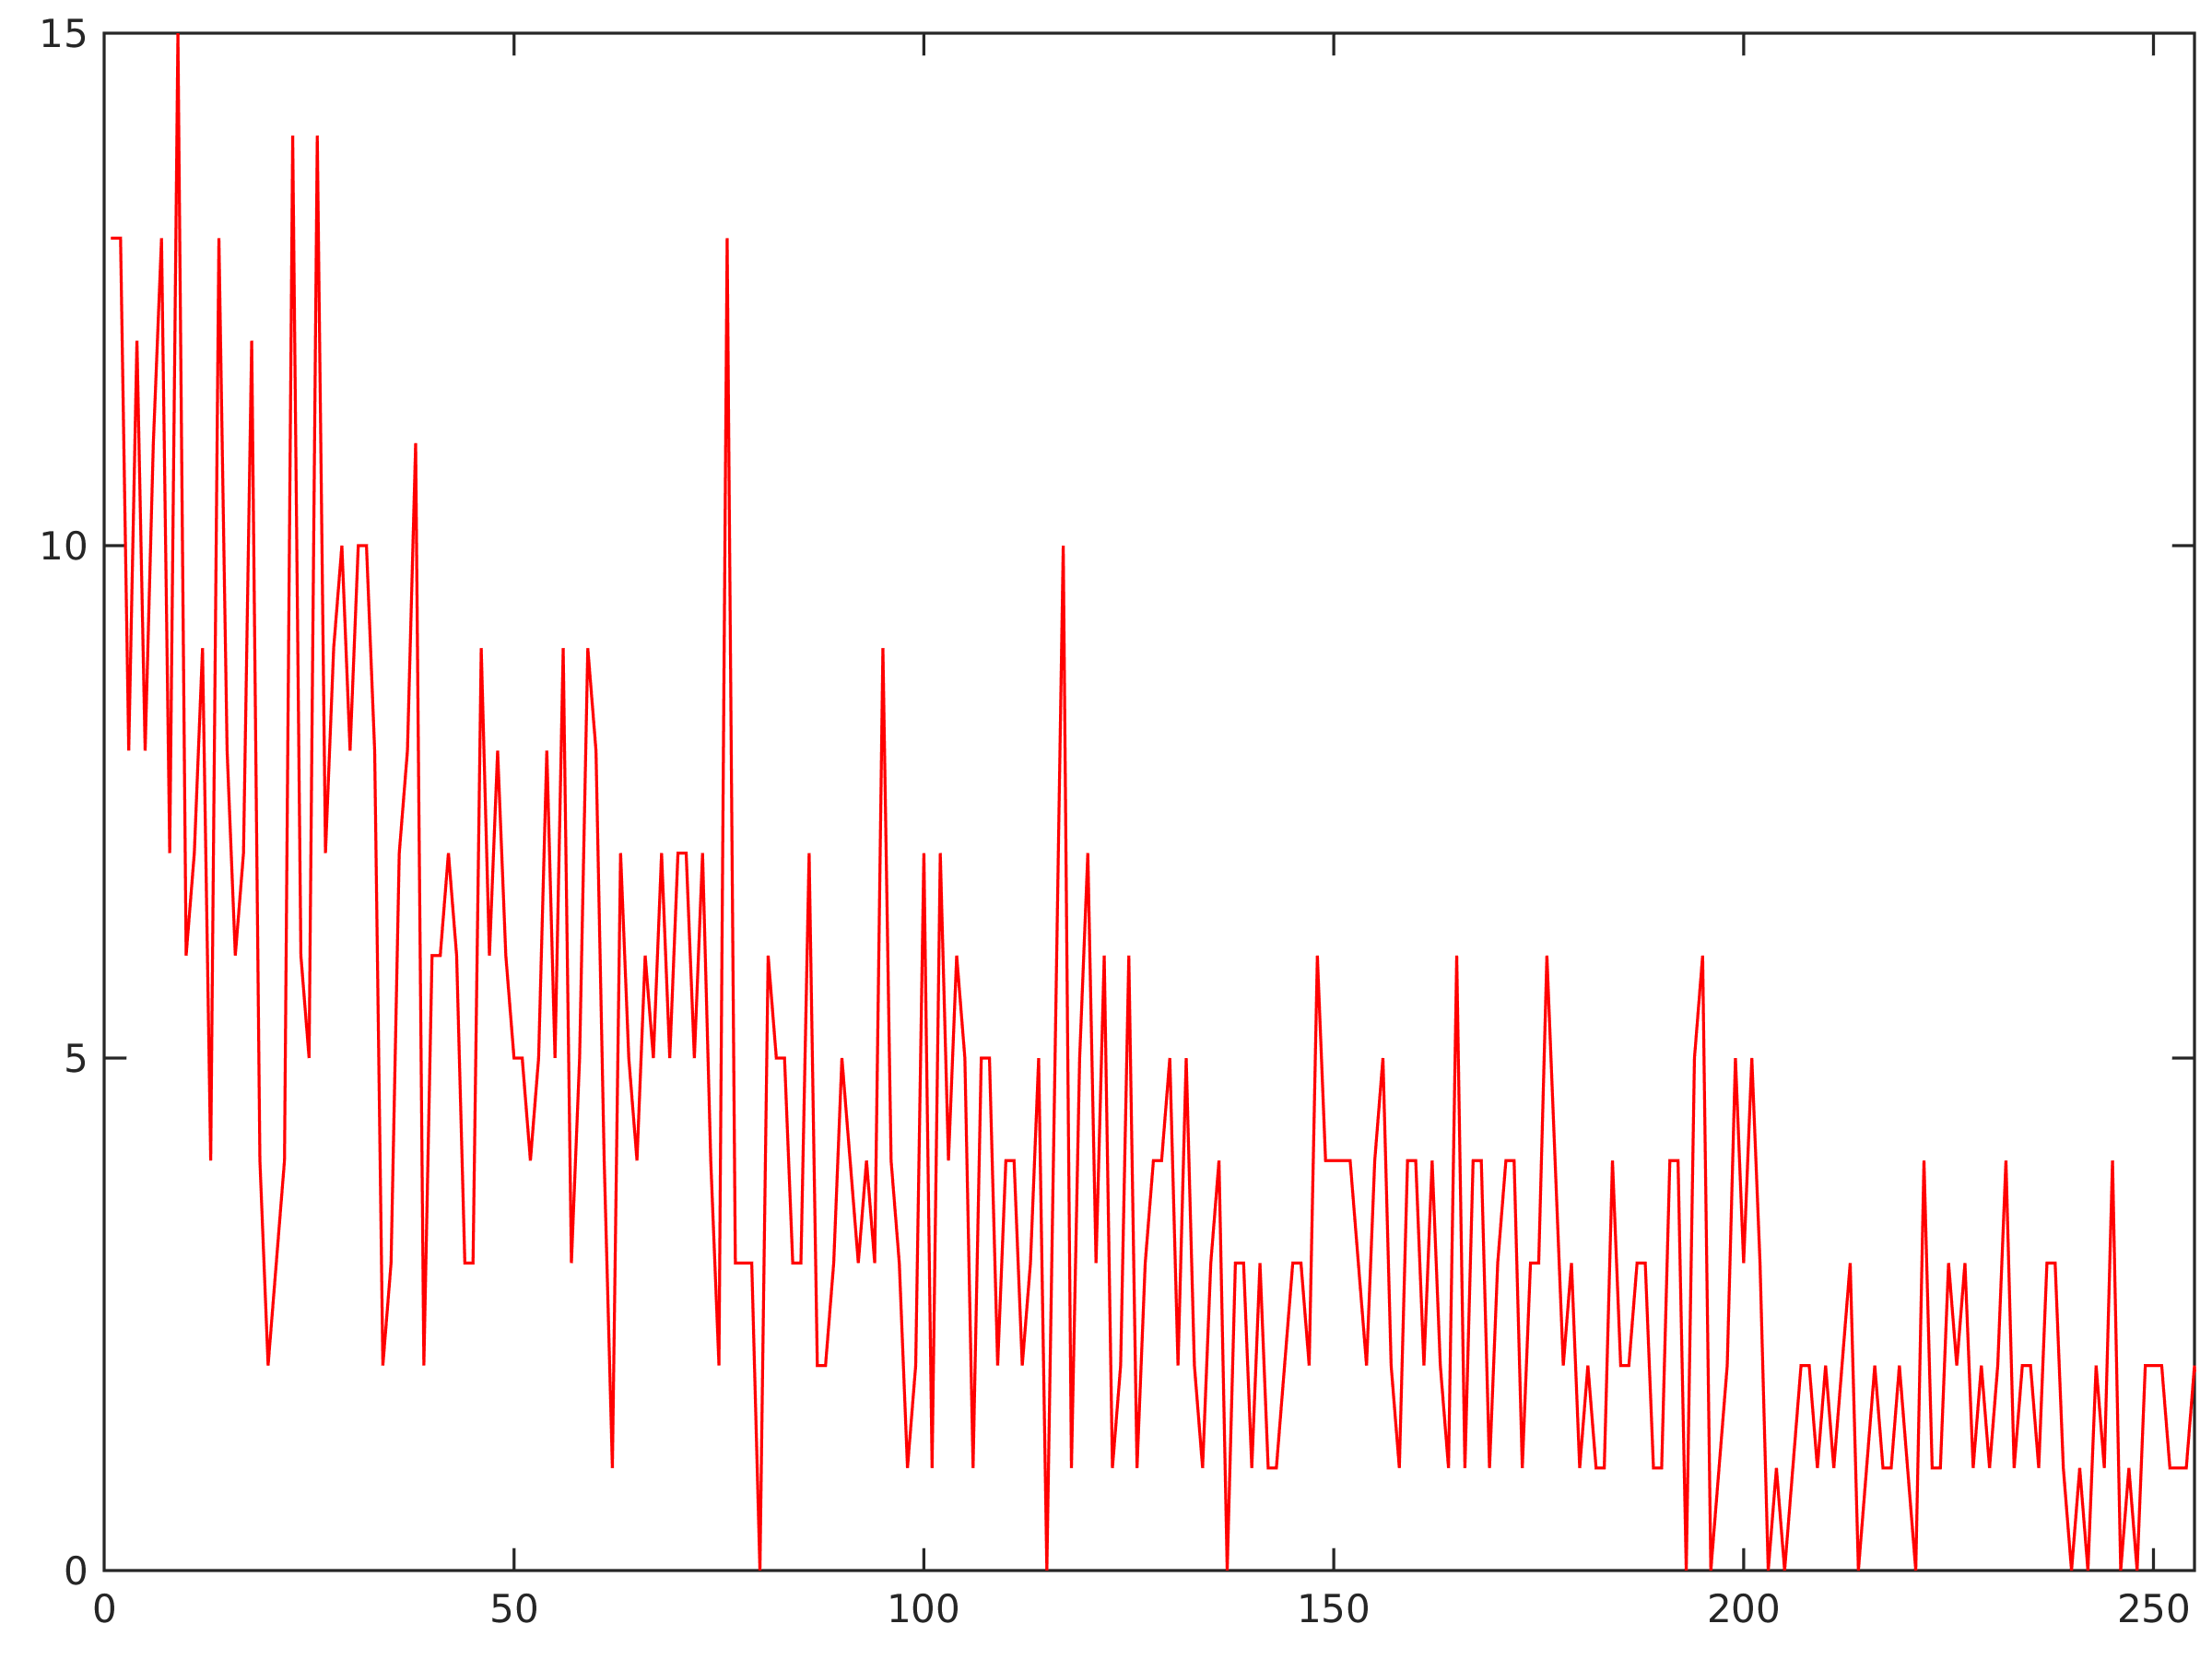
\includegraphics[width=0.25\textwidth]{2r}}
\subfigure{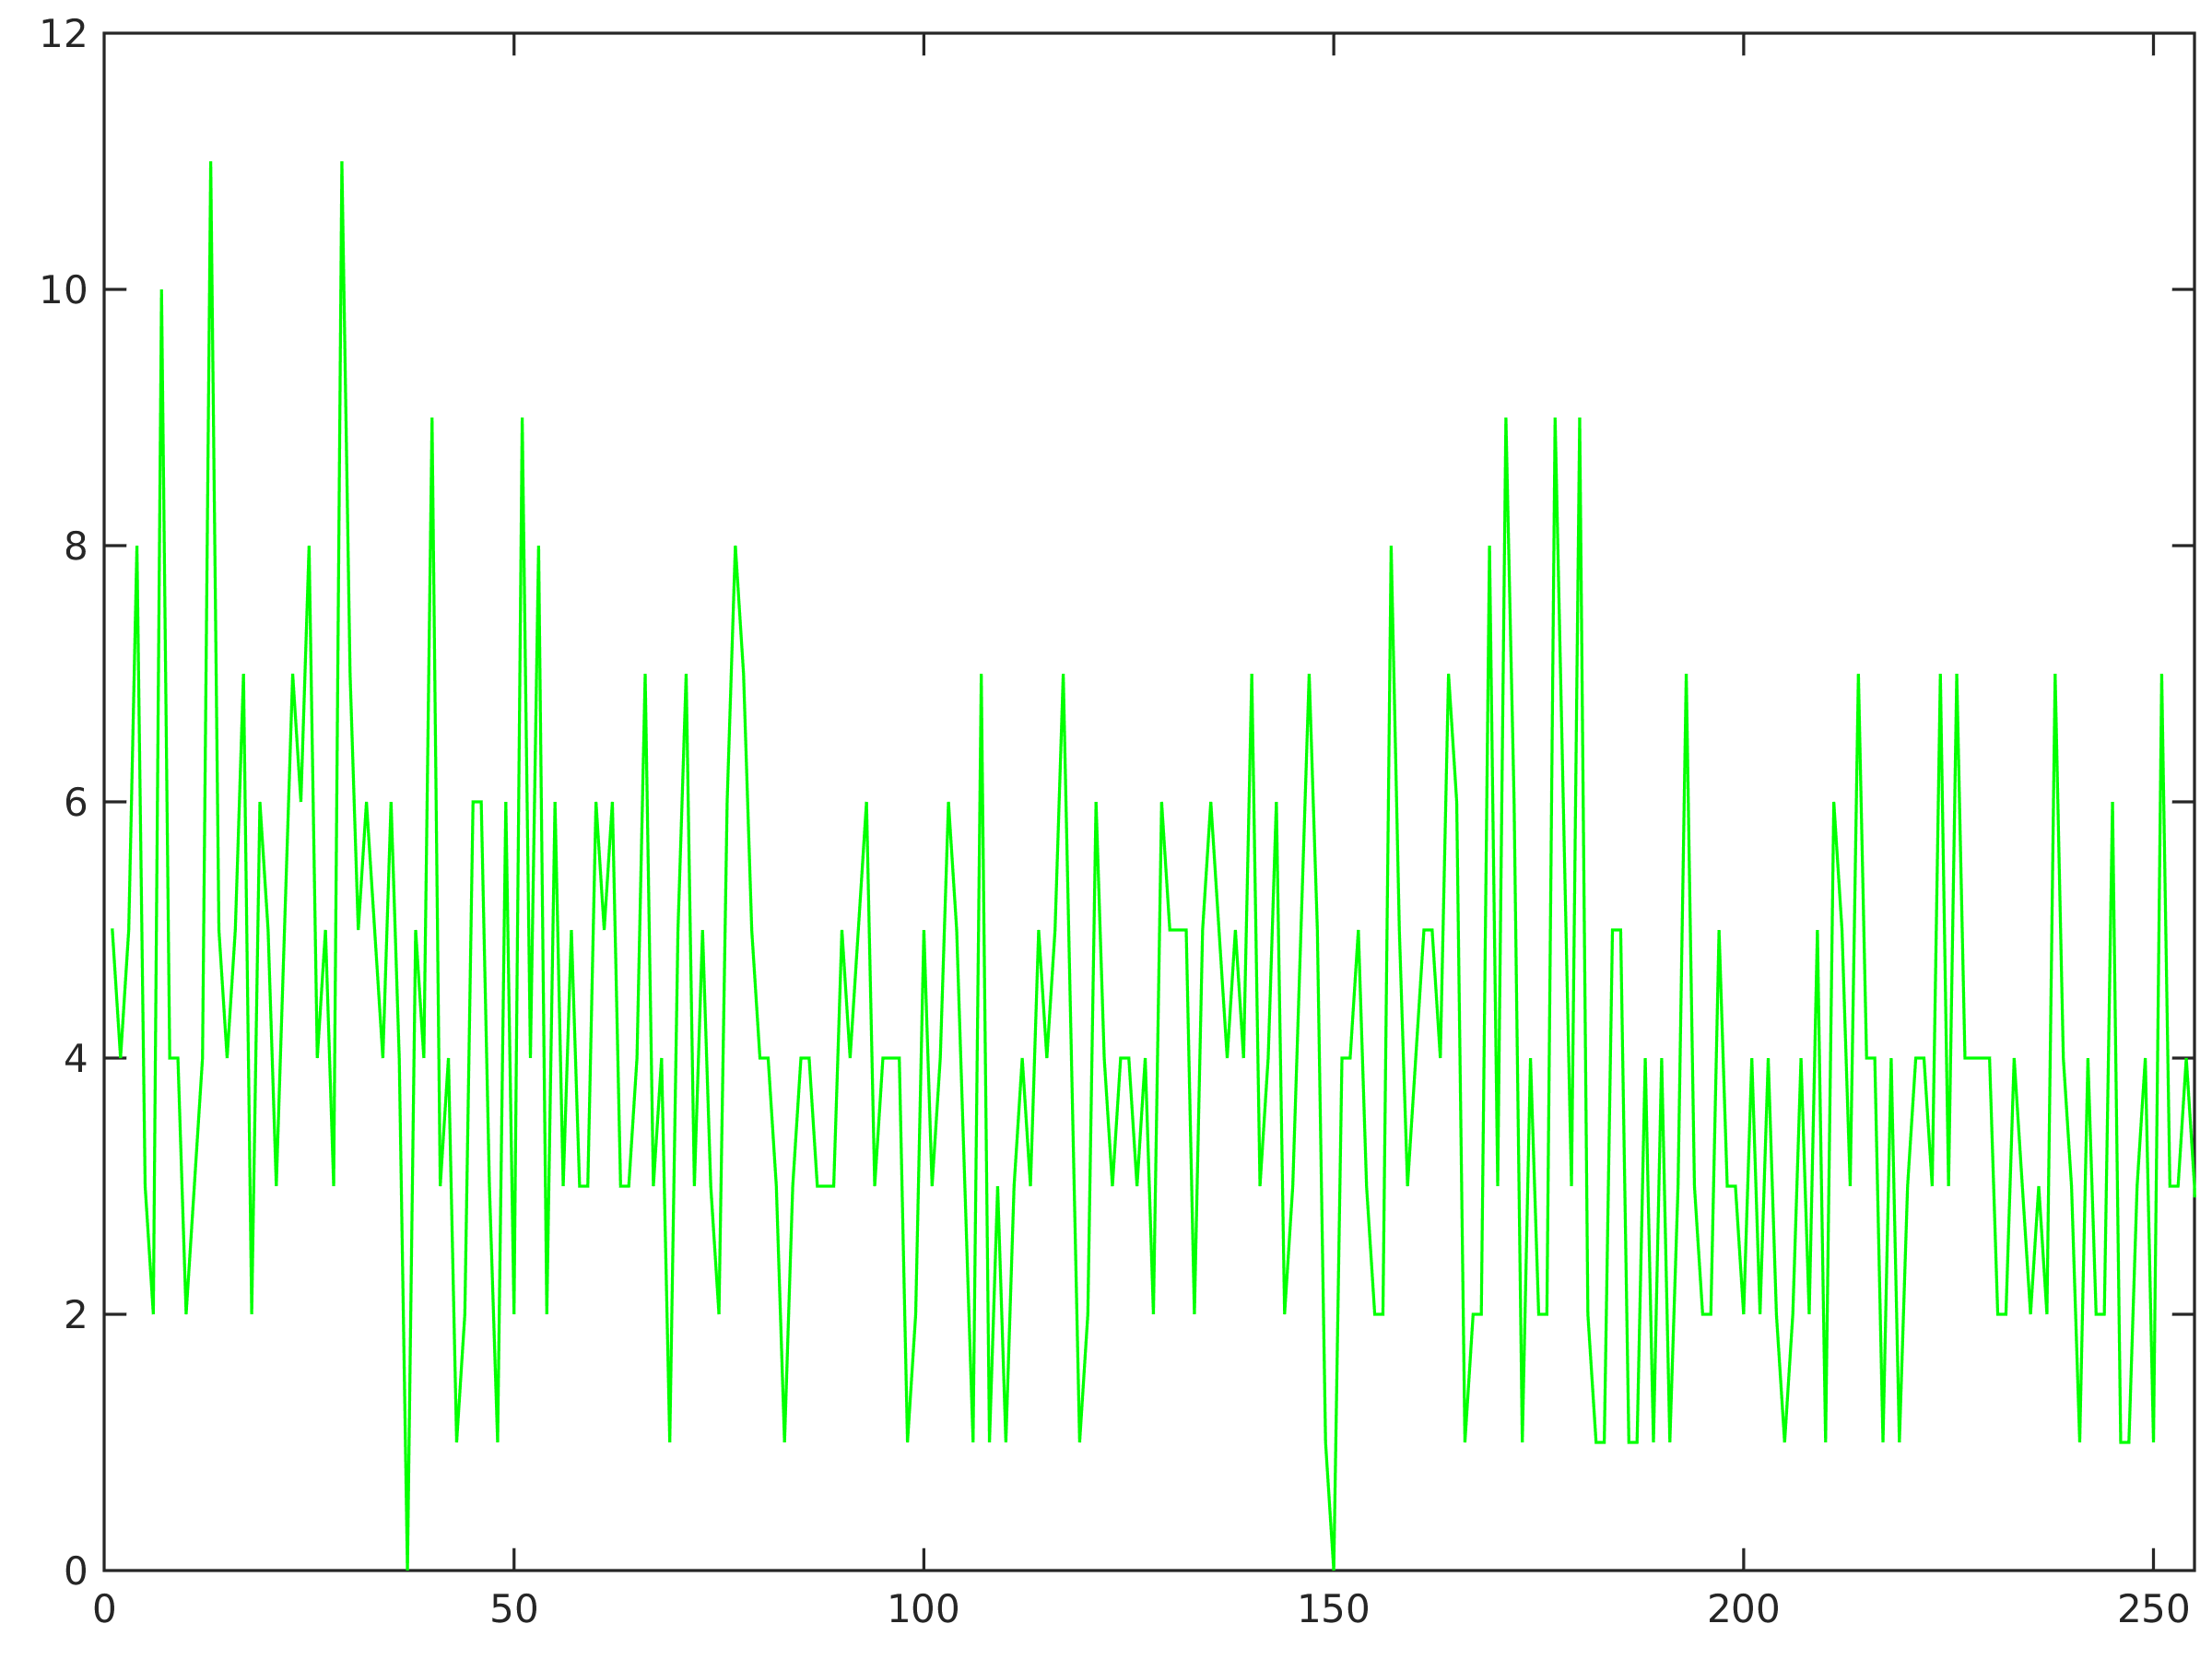
\includegraphics[width=0.25\textwidth]{2g}}
\subfigure{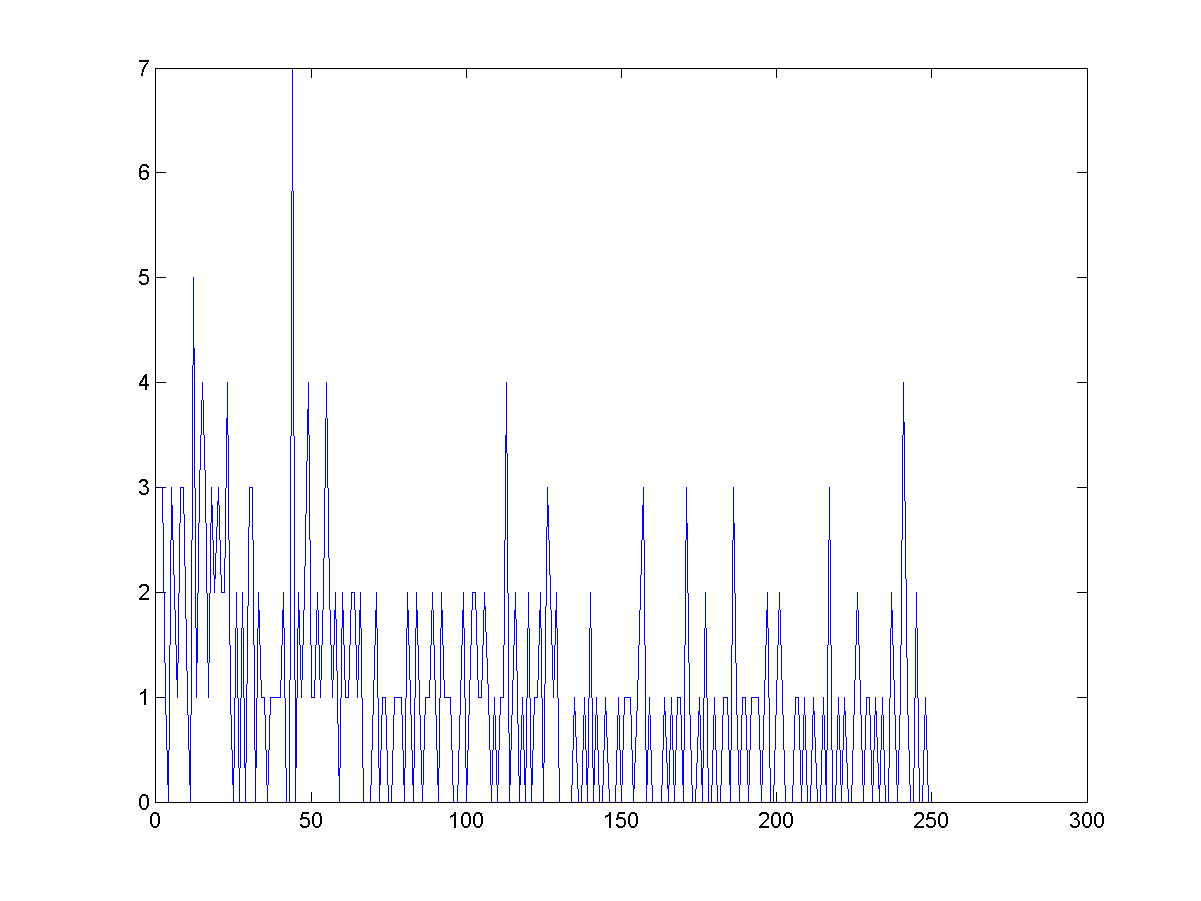
\includegraphics[width=0.25\textwidth]{2b}}
\subfigure[Label:-1 -1 1]{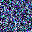
\includegraphics[width=0.2\textwidth]{3}}
\subfigure{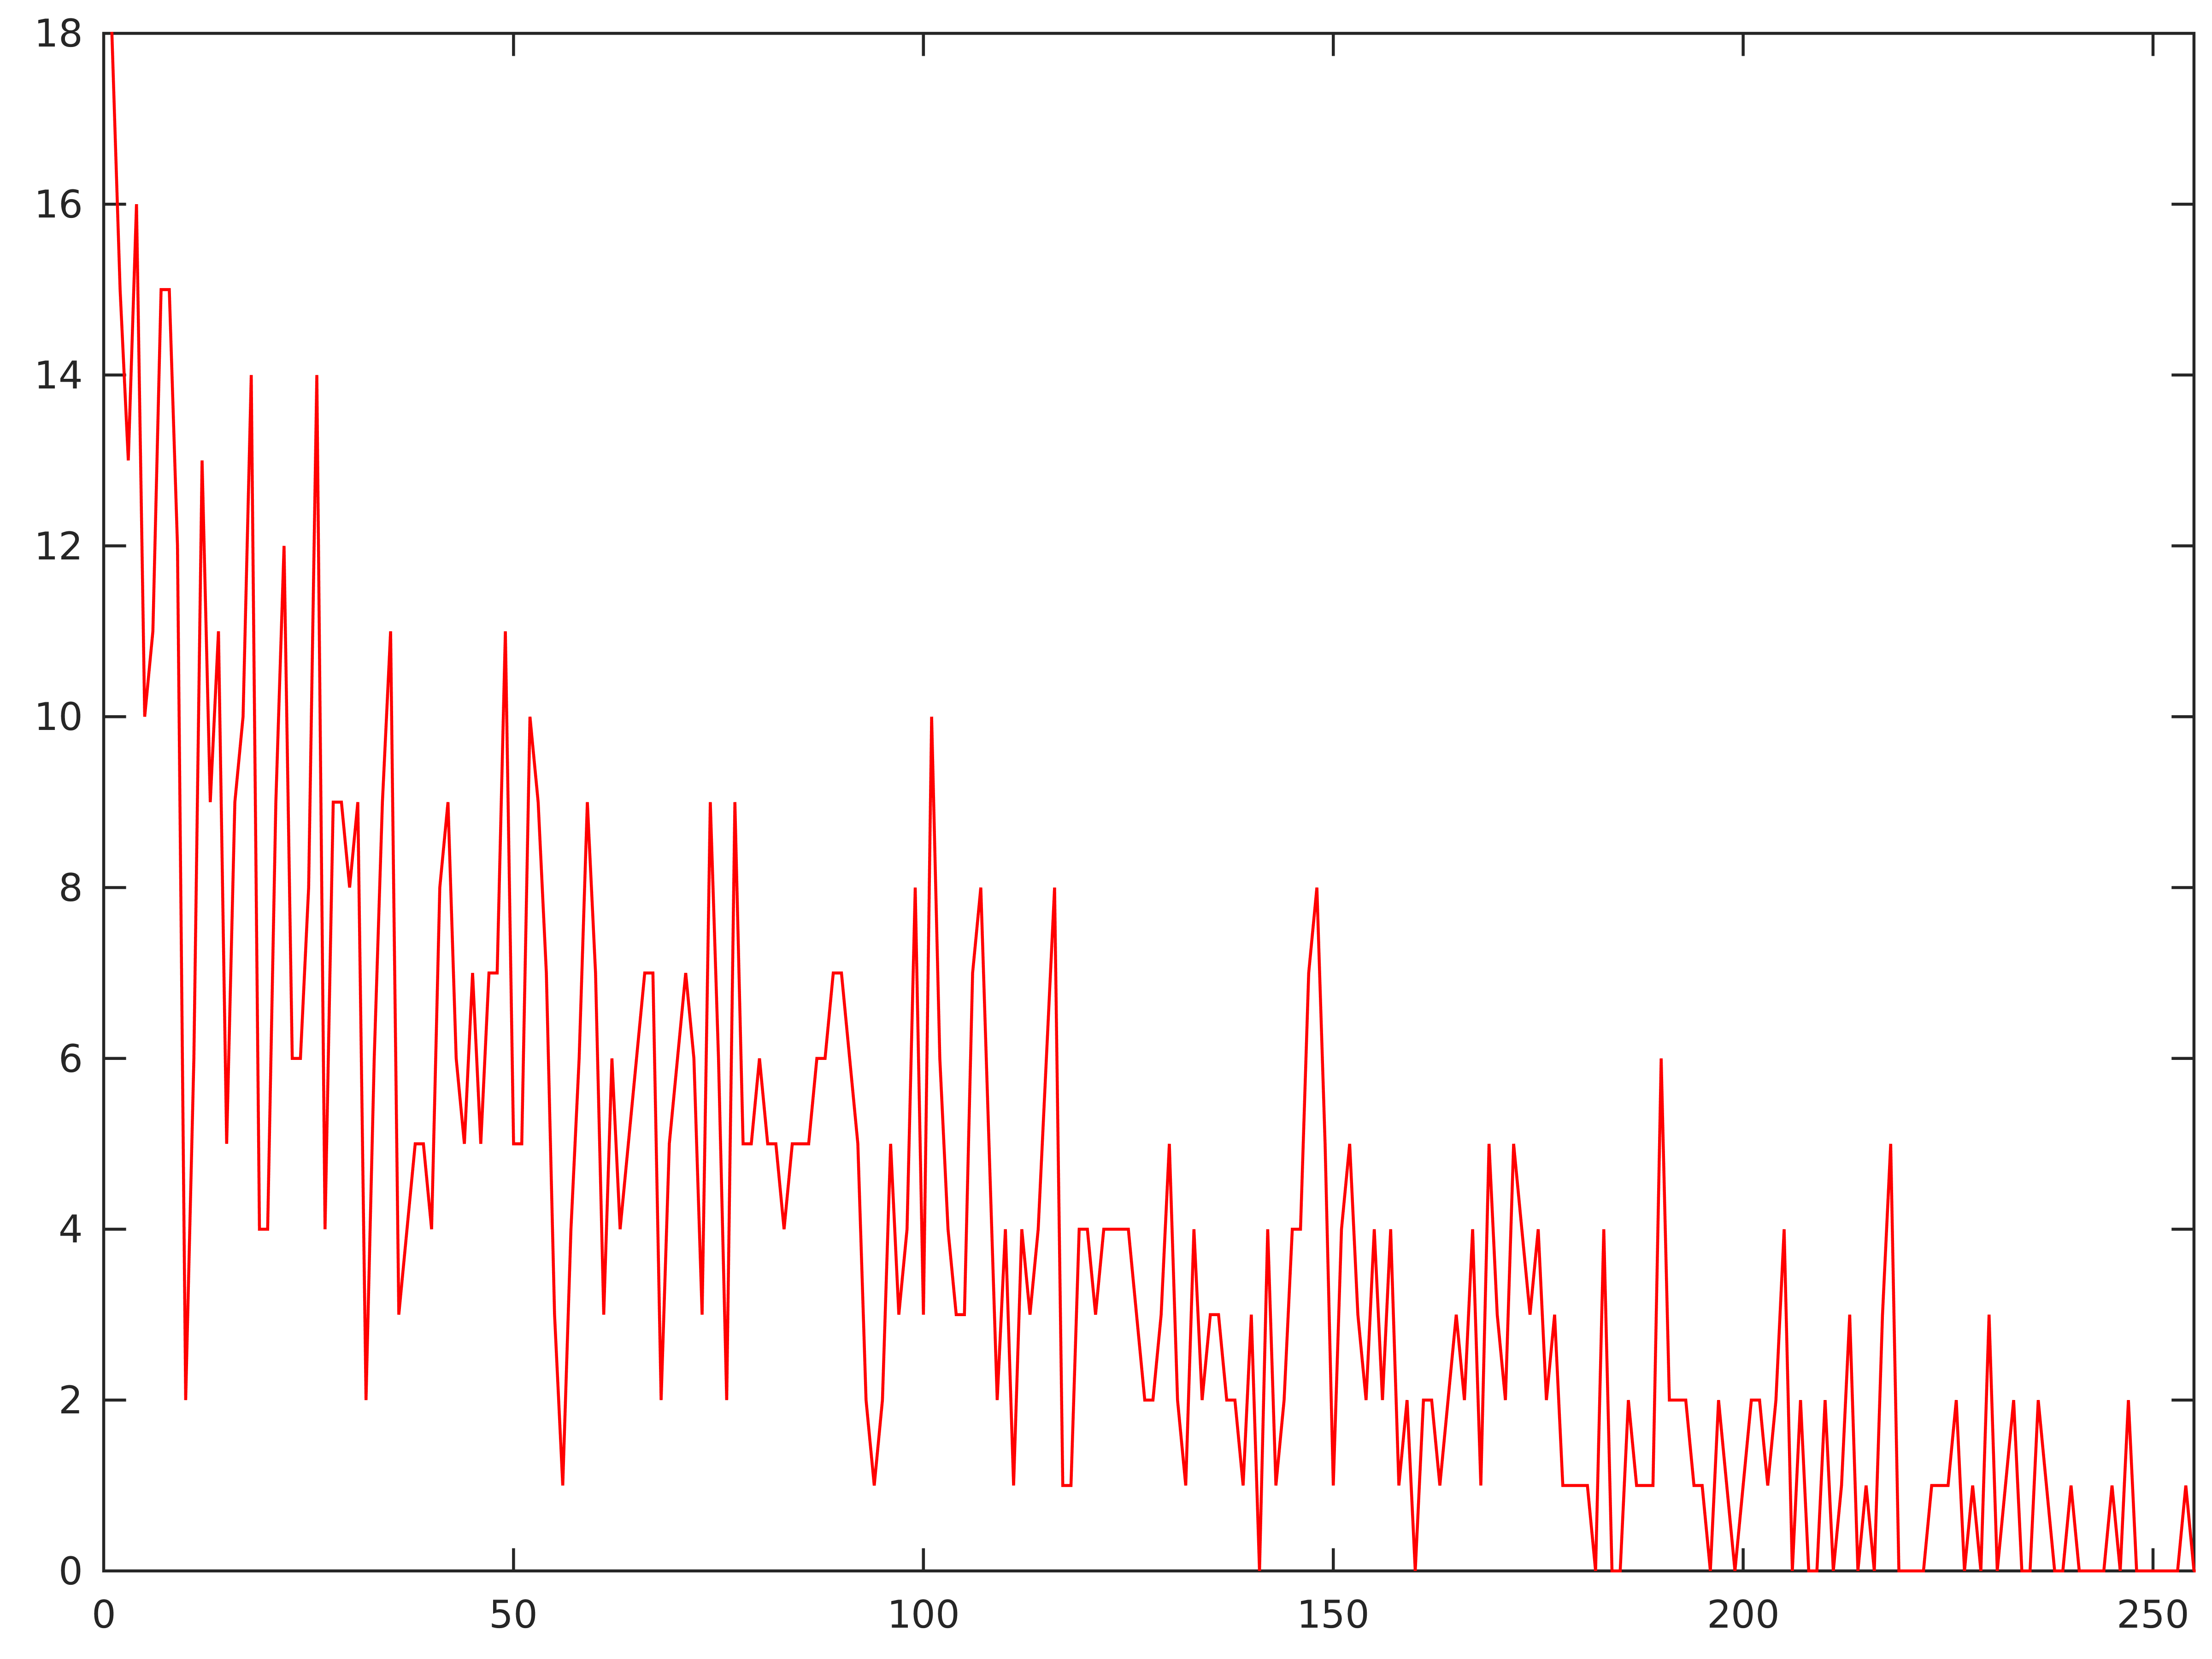
\includegraphics[width=0.25\textwidth]{3r}}
\subfigure{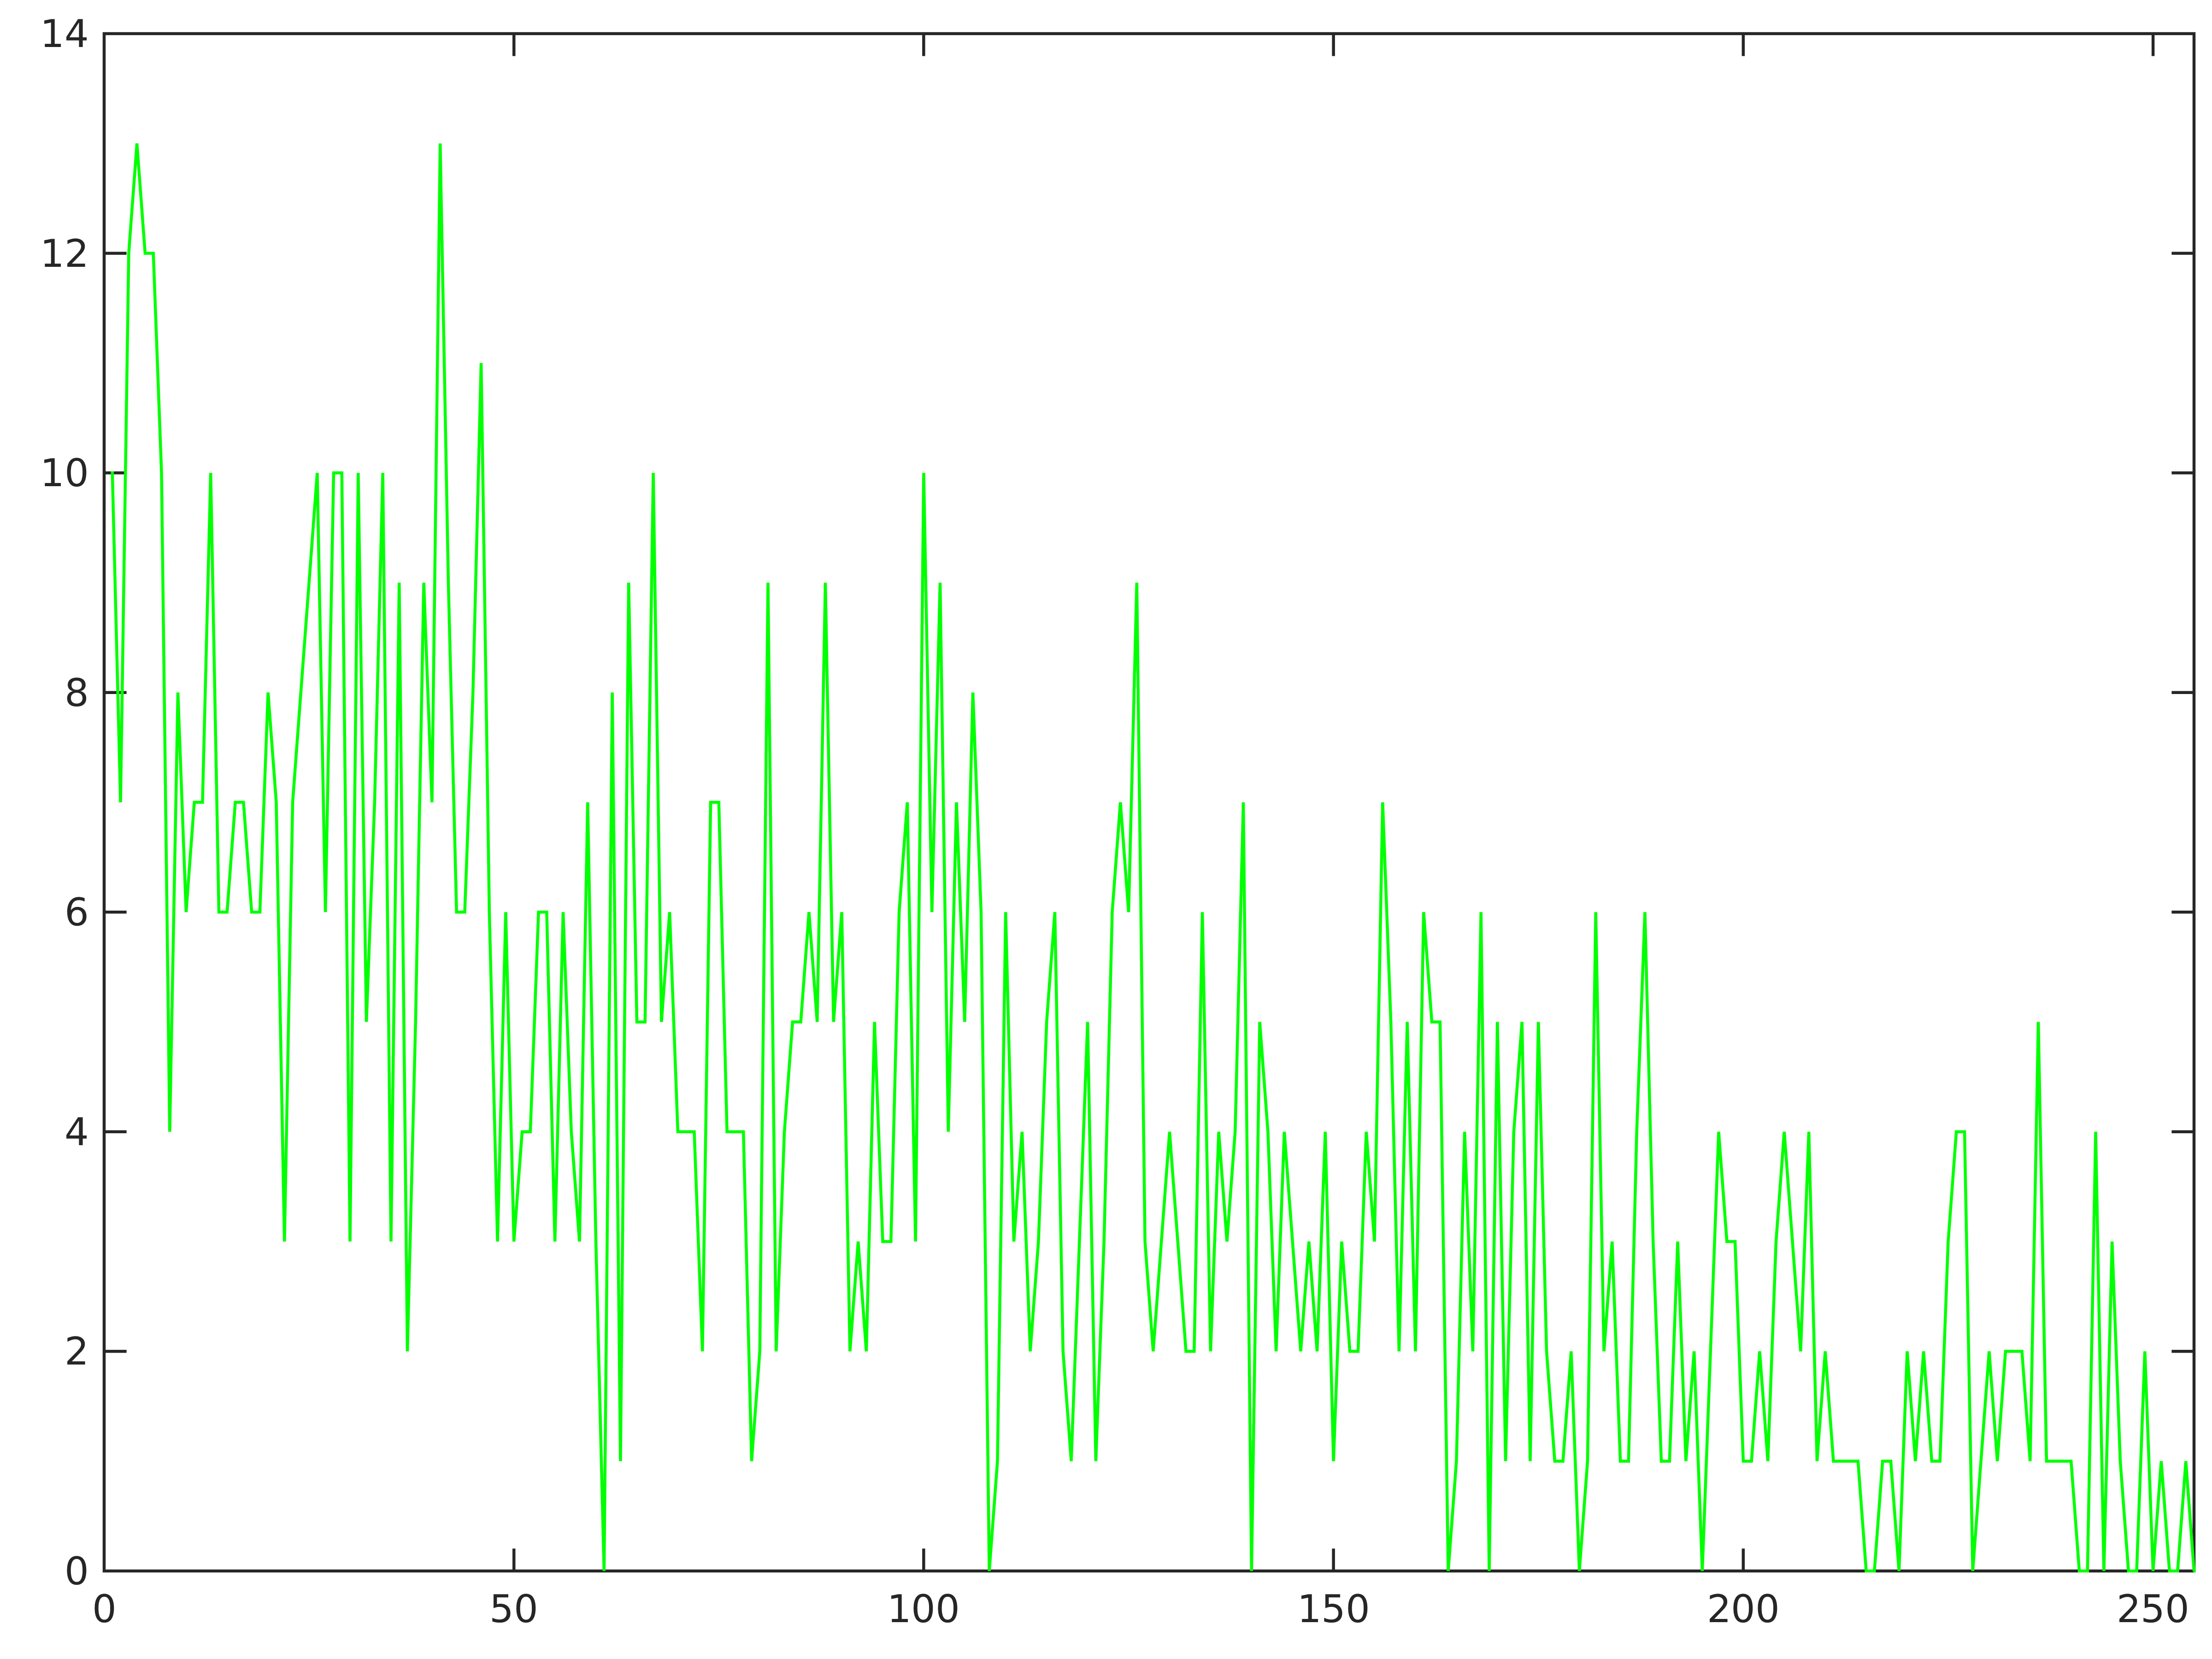
\includegraphics[width=0.25\textwidth]{3g}}
\subfigure{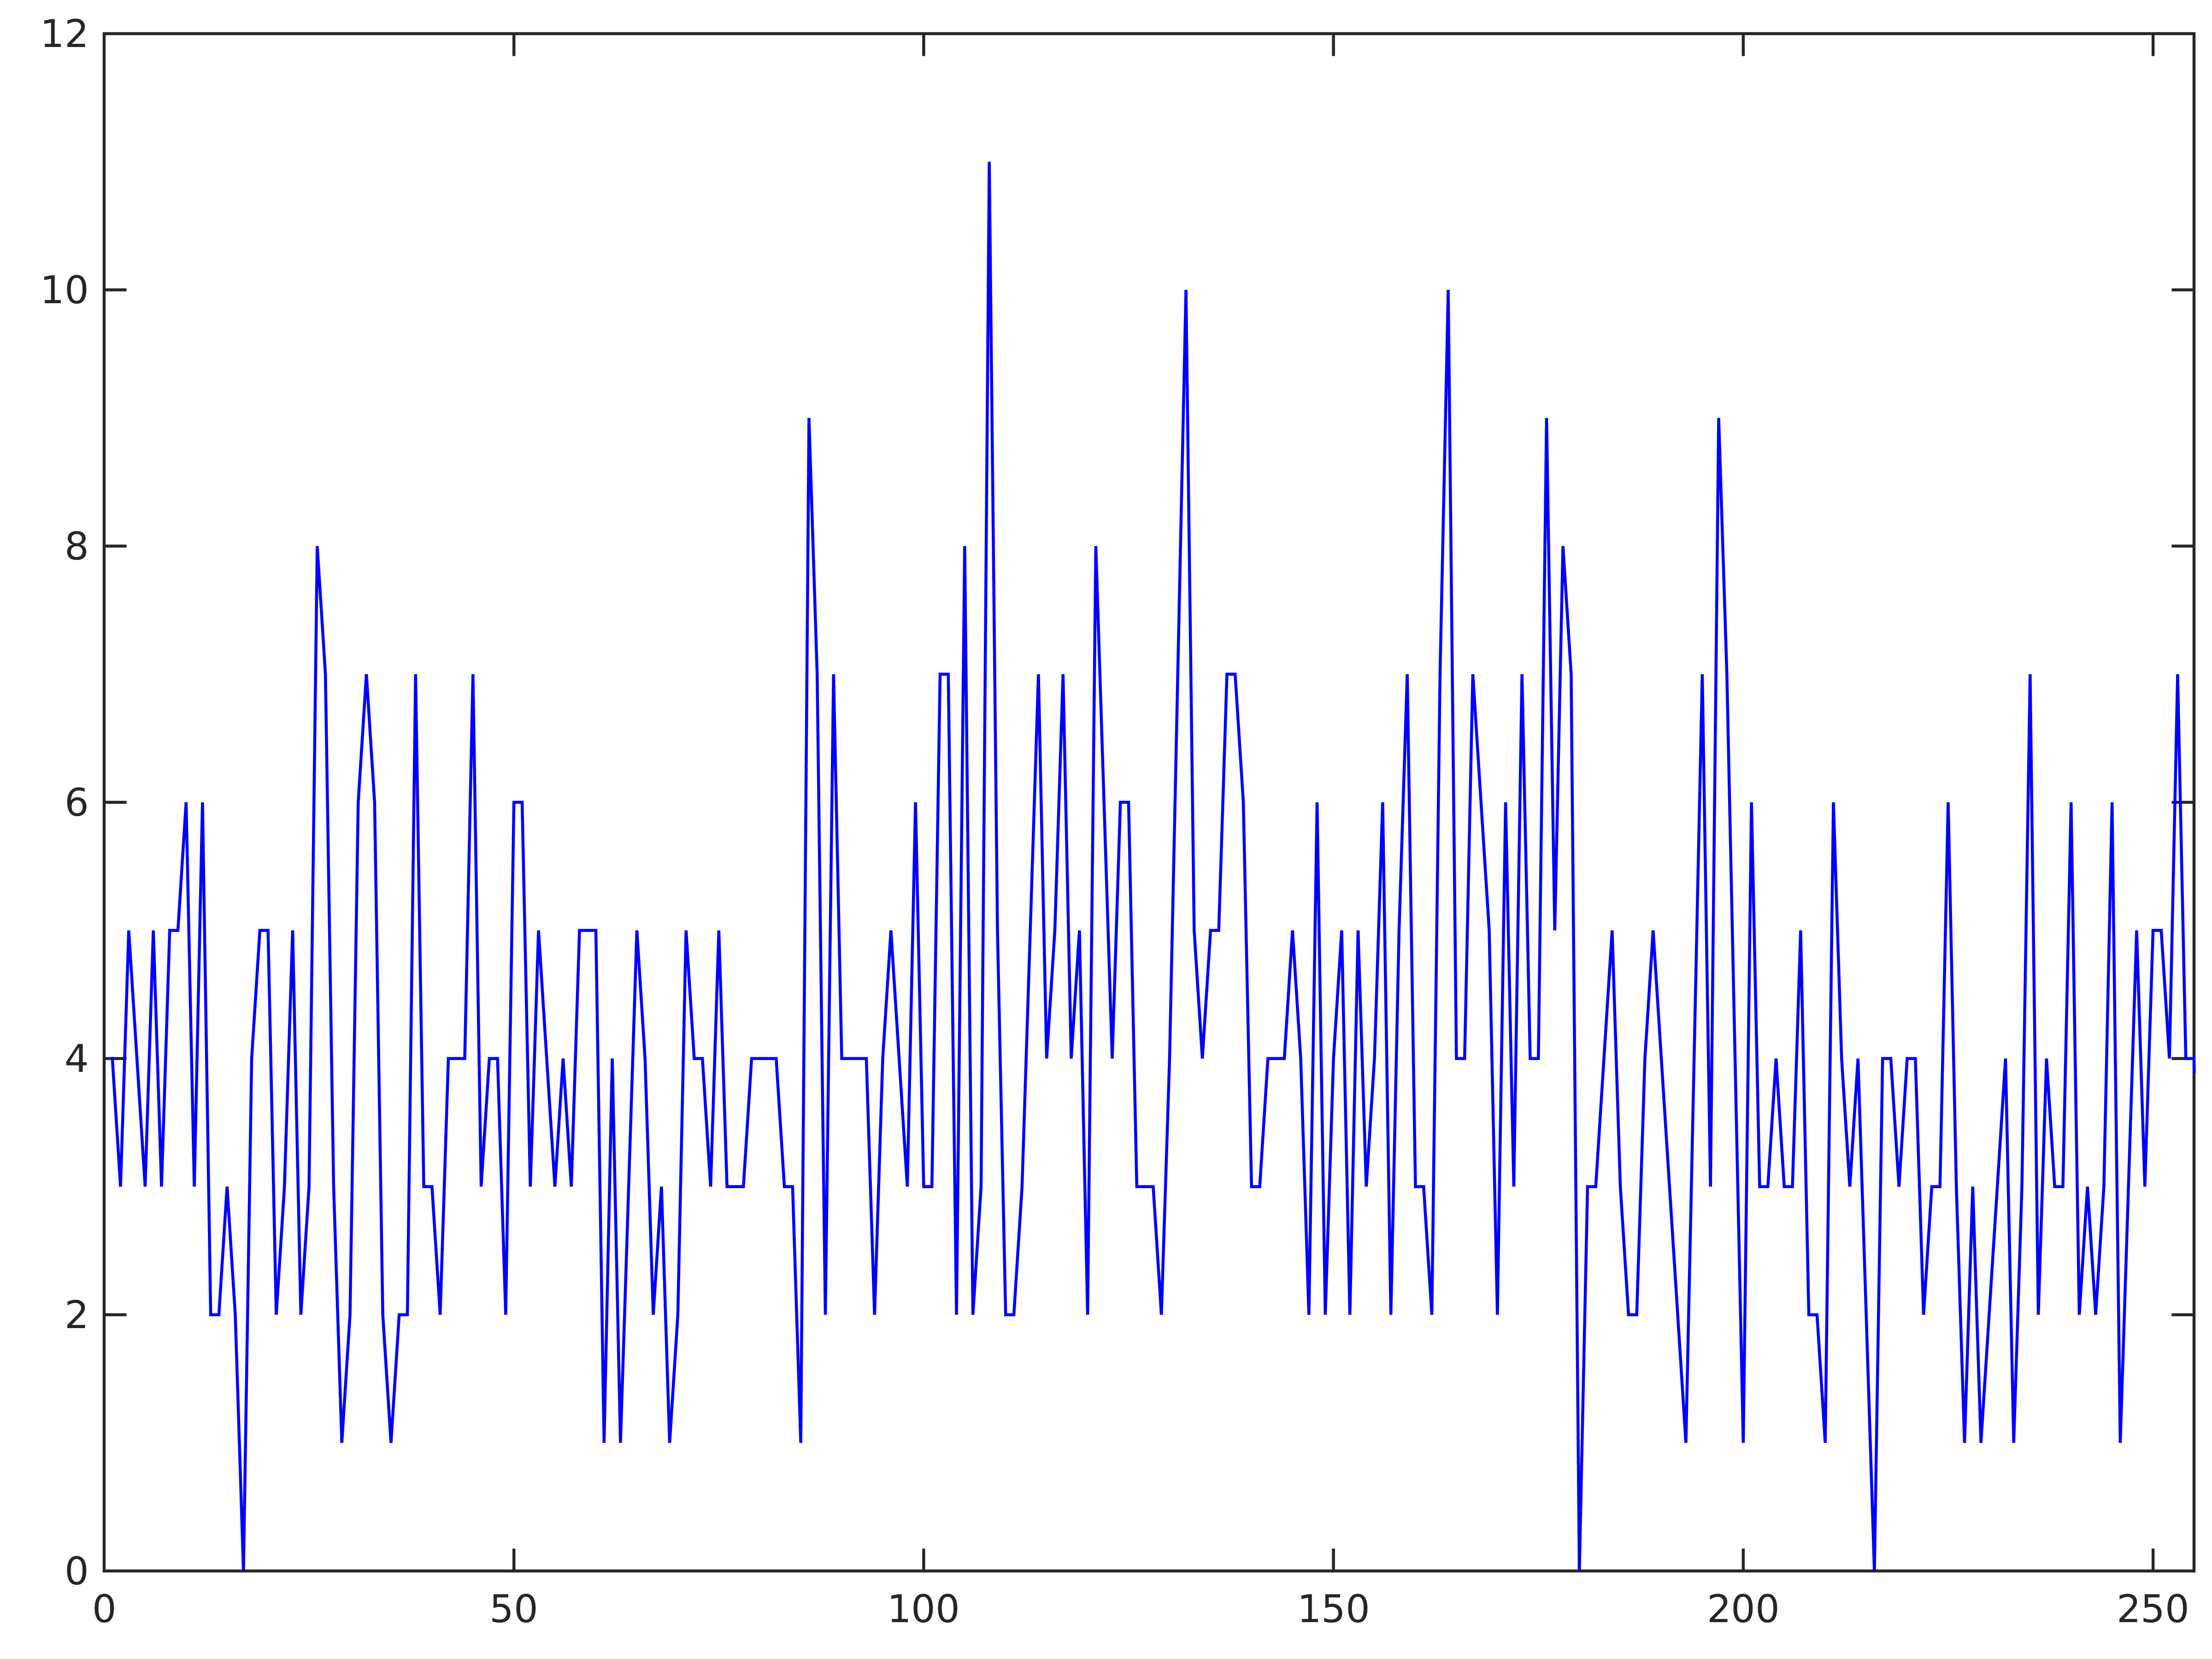
\includegraphics[width=0.25\textwidth]{3b}}
\caption{Multilabel samples and the RGB colour histograms. Three labels mean red, green and blue sequentially. }
\end{figure}

The dataset contains $1000$ images in total. $960$ images are training samples and $40$ are test samples. 

\section{Artificial Neural Network}

The Artificial Neural network is an approach to learning a nonlinear function which can be used to map samples to multi labels. The neurons in the first layer take a raw image while the neurons in the last layer produce outputs. Between the first and the last layers, the middle layers are called hidden layers because they do not connect to external world. A 3 layer neural network can represent any bounded degree polynomial under certain conditions\citep{barron1993universal}. The weights of neural network are learned by algorithms deployed over training dataset. One of successful learning algorithms is the Backpropagation algorithm which updates weights by propagating errors caused by comparing prediction for each sample with actual target values.

Two factors will be modified to adapt a neural network to do multi-label classification. One is to design a new error function which fits the characteristics of multi-label samples instead of single-label ones. The other is to find a moderate metric according to the new designed error function.

\subsection{Network Architecture}

Define $\mathcal{X} = \mathbb{R}^{d}$ as the sample space and $\mathcal{Y} = {1,2,...,Q}$ as the set of output labels. The training dataset is composed of $m$ multi-label samples, such as ${(x_{1}, Y_{1}),(x_{2}, Y_{2}),...,(x_{m}, Y_{m})}$, while each sample $x_{i} \in \mathcal{X}$ is represented as a $d$-dimensional feature vector and a set of $q$ labels associate with the sample. A network network, showed in figure \ref{fig:MultiLabelNet}, can be built up to learn a model .

\graphicspath{ {./Figures/} }
\begin{figure}[!htb]
\centering
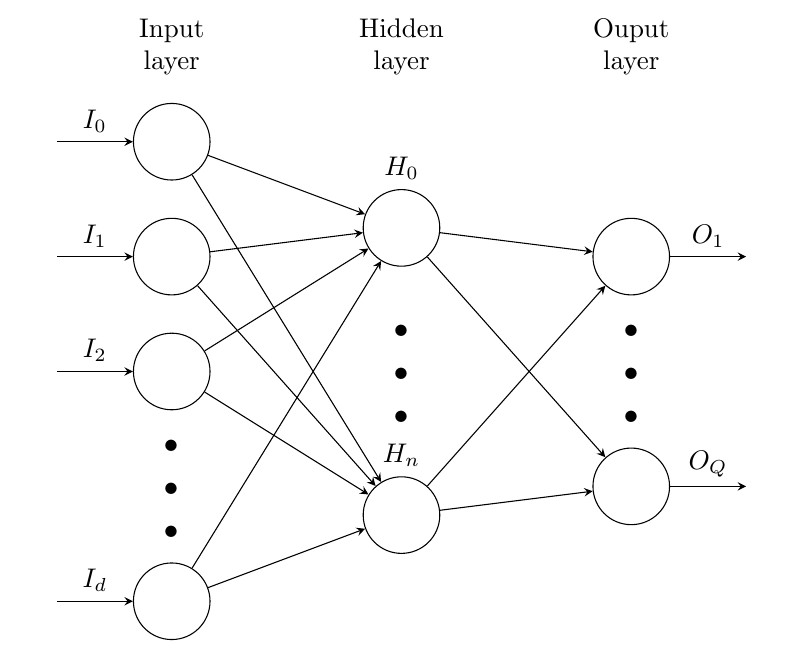
\includegraphics[width=0.8\textwidth]{MultiLabelNet.jpeg}
\caption{\label{fig:MultiLabelNet}Network Topology For Multi-lable classification}
\end{figure}

The network has $d$ input neurons which correspond to a $d$-dimensional feature vector, while last $Q$ neurons represent a combination of output labels. There is a hidden layer in figure \ref{fig:MultiLabelNet} which owns $n$ hidden neurons. The input layer is fully connected with hidden layer and the same connecting method is deployed between hidden layer and the output layer. So there are $d \times n$ weights $(W_{ih}, 1 \leq i \leq d, 1 \leq h \leq n)$ between the input layer and the hidden layer and $n \times q$ weights $(W_{ho}, 1 \leq h \leq n , 1 \leq o \leq q)$ between the hidden layer and the output layer. The bias parameters are represented as $I_{0}$ and  $H_{0}$.

Because the task of multi-label learning is to predict labels of test samples, it needs to evaluate the global error of the model as:
\begin{equation}\label{eq:MultiLableError}
E = \sum_{i=1}^m E_{i}
\end{equation}
$E_{i}$ is the error on sample $x_{i}$ which can be defined as:
\begin{equation}\label{eq:MultiLableSamError}
E_{i} = \sum_{j=1}^Q (c_{j}^i - d_{j}^i)^2
\end{equation}
where $c_{j}^i = c_{j}(x_{i})$ is the predicted $j$-th label by the model on sample $x_{i}$, and $d_{j}^i$ is the actual $j$-th label of sample $x_{i}$. The actual label has value of either $+1 (j \in \mathcal{Y_{i}})$ or $-1 (j \notin \mathcal{Y_{i}})$.

Various learning algorithms can be used to learn a model based on the training dataset. The Backpropagation(BP) algorithm is deployed to learn from errors. However, original BP algorithm could be improper in multi-label learning because the error function \ref{eq:MultiLableSamError} neglects the correlations among labels of a sample. In original BP algorithm, the error function \ref{eq:MultiLableSamError} limits on individual label discrimination, whether a specific label $j \in \mathcal{Y}$ belongs to the sample $x_{i}$ or not. It should take into consideration that labels in $Y_{i}$ are more important than those outside of $Y_{i}$. A new global error function is defined as:
\begin{equation}\label{eq:MultiLableGlobalError}
E = \sum_{i=1}^m E_{i} = \sum_{i=1}^m \frac{1}{|Y_{i}||\hat{Y}_{i}|} \sum_{(k,l) \in Y_{i} \times \hat{Y_{i}}} exp(-(c_{k}^i-c_{l}^i))
\end{equation}
In the error function \ref{eq:MultiLableGlobalError}, the $i$-th errors on the $i$-th sample $(x_{i},Y_{i})$ are accumulated. $\hat{Y}_{i}$ is complementary set of $Y_{i}$ in $\mathcal{Y}$ and $|\cdot|$ computes the cardinality of a set. Specifically, the item, $c_{k}^i-c_{l}^i$, represents the difference between the output labels of the model on a label which belongs to sample $x_{i}$ and a label which does not belong to the same sample. The error function\ref{eq:MultiLableGlobalError} shows that bigger difference leads to better performance. Additionally, the negation of the difference is put into the exponential function to sharply penalize the $i$-th term if $c_{k}^i$ is much smaller than $c_{l}^i$. The sum of $i$-th error term accumulates difference between outputs of any pair of labels which are the one belonging to the sample and the other one not belonging to it. The sum is normalized by the numbers of all pairs, $|Y_{i}||\hat{Y}_{i}|$. And then, the correlations between pair labels are computed. In the other words, labels in $Y_{i}$ should get larger output value than labels in $\hat{Y}_{i}$.

As previous statement, the error function \ref{eq:MultiLableGlobalError} calculates the difference between output labels. The task of learning is minimizing the error function \ref{eq:MultiLableGlobalError} via enlarging output values of labels belonging to the training samples and diminishing the output values of the labels not belonging to it. If the training dataset can cover the distribution of the whole sample space, neural network model can learn it through minimizing error function by feeding training samples.

\subsection{Error Function}

The basic goal of regression problems is to figure out the conditional distribution of the output labels, given the input samples. It is common to use a sum-of-squares error function.

The basic goal of classification problems is to figure out the posterior probabilities of class types, given the input samples. Except for sum-of-squares error function, there are some more approximate error functions which can be considered.

The central goal in training a neural network is to model the hidden generator of the samples instead of memorizing the training samples. Therefore, the best prediction of an input sample can be found if the network can present a new value for the sample. Because the general and complete characterization of the generator of the dataset is the probability density $p(x,t)$. It is available to decompose a joint probability density into the product of the conditional density of the labels, the input data and the density of input data,
\begin{equation}\label{eq:JointProbDensity}
p(x,t) = p(t|x)p(x)
\end{equation}
where $p(t|x)$ represents the probability density of $t$ if $x$ is a distinct label and $p(x)$ represents the density of $x$
\begin{equation}\label{eq:ProbDensityX}
p(x) = \int p(t,x)dt
\end{equation}

Most error functions can be obtained from the idea of maximum likelihood. For training dataset, 
\begin{equation}\label{eq:LikelihoodLoss}
L = \coprod_{\substack{n}}  p(t^n|x^n)p(x^n)
\end{equation}
where each sample is picked out randomly from the same  distribution and their probabilities can be multiplied. The error function can be represented by minimizing the negative logarithm of the likelihood since the negative logarithm is a monotonic function.
\begin{equation}\label{eq:LikelihoodErrorFunc}
E = -ln L = -\sum_{\substack{n}} ln p(t^n|x^n) - \sum_{\substack{n}}lnp(x^n)
\end{equation}
where $E$ is notated as an error function. The task of the neural network is to model the conditional probability density $p(t|x)$. And the second term is independent with the parameters in neural networks.  We can simplify \ref{eq:LikelihoodErrorFunc} to
\begin{equation}\label{eq:SimLikelihoodErrorFunc}
E = -ln L = -\sum_{\substack{n}} ln p(t^n|x^n) + C
\end{equation}
It is worth noting that error functions are dependent on different assumptions of the forms of the conditional distribution $p(t|x)$. In this classification task, $t$ represents labels which act as class members or the prediction of the probabilities of class members.

\subsection{Cross Entropy}

The Mean Square Error is a common risk metric comparable to the predicted value of the squared error loss. It is simple to implementation and non-negative. However, it has the disadvantage of heavily weighting outliers\citep{bermejo2001oriented}.

Given that there are two discrete distributions $p(x)$ and $q(x)$ over the same variable $x$. The relative entropy, relating to cross entropy, is a measurement of the distance between samples:
\begin{equation}\label{eq:RelativeEngtropy}
D_{pq}(p(x), q(x)) = \sum_{\substack{x}}q(x)ln\frac{q(x)}{p(x)}
\end{equation}
where the relative entropy is not a true metric because \ref{eq:RelativeEngtropy} could not be symmetric in the interchange $p \leftrightarrow q$ and probably not satisfy the triangle inequality.

Cross entropy loss, also named logistic regression loss, is an alternative measurement of a probability distribution. The measure is commonly used in neural networks. It can be used to evaluate the posterior probabilities of class membership.

Given that training a neuron, which has several input data, $x_{1}, x_{2},...,$ with weights $w_{1}, w_{2},...,$ and a bias, $b$, the outputs, for example two classes, can be represented as the weighted sum of the input data.
\begin{equation}\label{eq:EquationNN}
a = f(x) = \sum_{i}w_{i}x_{i} + b
\end{equation}
Then the cross entropy cost function is
\begin{equation}\label{eq:TwoClassCrossEntropyCostFunc}
C = -\frac{1}{n} \sum_x \left[y \ln a + (1-y ) \ln (1-a) \right]
\end{equation}
where $n$ is the number of training samples, $a$ is the prediction result and $y$ is actual result.

The cross entropy can act as a cost function because of two properties. First, $C$ is non-negative, because the items of logarithms are in the range $[0,1]$ and there is a minus sign at the beginning of the sum. Second, if the prediction output is close to the actual value for all training samples, the loss value, $C$, will be close to $0$. Given that $y = 0$ and the prediction value $a \approx 0$, the first item in \ref{eq:TwoClassCrossEntropyCostFunc} is $0$ while the second item is $-\ln(1-a) \approx 0$. The similar situation occurs for situation, $y = 1$ and $a \approx 1$. Therefore, the value of cost function will be small, if the prediction value is close to the actual value.

In total, the cross entropy tends to $0$, when the neuron acts better at predicting the output $y$ for total training inputs $x$. The two properties are basic to a cost function. Although the quadratic cost function satisfy the properties, the cross entropy has the advantage on avoiding the issue of learning curve slowing down. To illustrate the advantage, the partial derivative of the cross entropy cost function can be done with the respect to the weights. Applying the chain rule twice on \ref{eq:TwoClassCrossEntropyCostFunc}
\begin{eqnarray}\label{eq:DerCrossEntropyCostFunc}
  \frac{\partial C}{\partial w_j} & = & -\frac{1}{n} \sum_x \left(
    \frac{y }{f(x)} -\frac{(1-y)}{1-f(x)} \right)
  \frac{\partial f}{\partial w_j} \\
 & = & -\frac{1}{n} \sum_x \left( 
    \frac{y}{f(x)}-\frac{(1-y)}{1-f(x)} \right)f'(x) x_j.
\end{eqnarray}
where the second equation can be represented as
\begin{equation}\label{eq:SecondDerCrossEntropyCostFunc}
  \frac{\partial C}{\partial w_j} = \frac{1}{n}  \sum_x \frac{f'(x) x_j}{f(x) (1-f(x))} (f(x)-y)
\end{equation}
Because the defination of the sigmoid function is $f(x) =1/(1+e^{-x})$ and the derivative of sigmoid function is $f'(x) =f(x)(1-f(x))$. Then the items $f'(x)$ and $f(x) =1/(1+e^{-x})$ cancel in the equation and it becomes
\begin{equation}\label{eq:SimDerCrossEntropyCostFunc}
 \frac{\partial C}{\partial w_j} =  \frac{1}{n} \sum_x x_j(f(x)-y)
\end{equation}
The equation shows that the rate of learning weights is controlled by $f(x) - y$. The larger the error is, the faster the neuron learns. In particular, the property avoids the learning slowdown because the derivative item $f'(x)$ gets canceled out in the quadratic cost.

In the similar way, the bias can be computed by the partial derivative.
\begin{equation}\label{eq:BiasCrossEntropyCostFunc}
\frac{\partial C}{\partial b} = \frac{1}{n} \sum_x (f(x)-y)
\end{equation}


\subsection{Training and Testing}

Following the training process, gradient descent is used to minimize the global error function with backpropagation. 

To train a sample $(x_{i}, Y_{i})$, in which $x_{i}$ is the input data and $Y_{i}$ is the associated label, the predicted output labels computed by the neural network for is
\begin{equation}\label{eq:MultiLabelActivation}
c_{k} = f(netc_{k} + \theta_{k})
\end{equation}
where $\theta_{k}$ is the bias units of $k$ layer, $f()$ is the activation function of the output neurons which is a $tanh$ function\ref{eq:tanh} in this project. $netc_{k}$ is the input data of the layer:
\begin{equation}\label{eq:MultiLabel}
netc_{k} = \sum_{s=1}^M b_{s}w_{sk}
\end{equation}
where $w_{sk}$ is the weights for layers $s$ and $k$, while $M$ is the number of neurons in the hidden layer.

As $tanh$ function is differentiable, the general error of the $k$-th output neuron can be defined:
\begin{equation}\label{eq:MultiLableErrorDif}
d_{k} = -\frac{\partial E}{\partial netc_{k}}
\end{equation}
combining with \ref{eq:MultiLabelActivation}, we can get
\begin{equation}\label{eq:MultiLableChainRule}
d_{k} = -\frac{\partial E_{i}}{\partial c_{j}} \frac{\partial c_{j}}{\partial netc_{k}} = - \frac{\partial E_{i}}{\partial c_{j}} f'(netc_{k} + \theta_{k})
\end{equation}
With considering global error function \ref{eq:MultiLableGlobalError}
\begin{equation}\label{eq:MultiLablePartialC}
\frac{\partial E_{i}}{\partial c_{j}}= 
\begin{cases}
    -\frac{1}{|Y_{i}||\hat{Y}_{i}|} \sum_{l \in \hat{Y}_{i}} exp(-(c_{j} - c_{l}))       & \quad \text{if } j \in Y_{i}\\
    \frac{1}{|Y_{i}||\hat{Y}_{i}|} \sum_{k \in Y_{i}} exp(-(c_{k} - c_{j}))       & \quad \text{if } j \in \hat{Y}_{i}\\
  \end{cases}
\end{equation}
with derivation of $tanh$, and substituting it with \ref{eq:MultiLableChainRule} and \ref{eq:MultiLablePartialC} we can get
\begin{equation}\label{eq:MultiLableGenErr}
d_{k}= 
\begin{cases}
    \big(-\frac{1}{|Y_{i}||\hat{Y}_{i}|} \sum_{l \in \hat{Y}_{i}} exp(-(c_{j} - c_{l}))\big)(1+c_{j})(1-c_{j})       & \quad \text{if } j \in Y_{i}\\
    \big(\frac{1}{|Y_{i}||\hat{Y}_{i}|} \sum_{k \in Y_{i}} exp(-(c_{k} - c_{j}))\big)(1+c_{j})(1-c_{j})       & \quad \text{if } j \in \hat{Y}_{i}\\
  \end{cases}
\end{equation}
According to the previous method, we can define the general error of the $s$-th hidden neuron:
\begin{equation}\label{eq:MultiLableGenErrS}
e_{s} = - \frac{\partial E_{i}}{\partial netb_{s}}
\end{equation}
with $b_{s} = f(netb_{s} + \lambda_{s})$ and chain rule,
\begin{equation}\label{eq:MultiLablePartialE}
e_{s} = - \frac{\partial E_{i}}{\partial b_{s}} \frac{\partial b_{s}}{\partial netb_{s}} = - \big( \sum_{j=1}^Q \frac{\partial E_{i}}{\partial netc_{j}} \frac{\partial netc_{j}}{\partial b_{s}}\big)f'(netb_{s} + \lambda_{s})
\end{equation}
For $d_{j} = - \frac{\partial E_{i}}{\partial netc_{j}}$ and $netc_{j} = \sum_{s=1}^M b_{s}w_{sj}$, then 
\begin{equation}\label{eq:MultiLableGenErrEs}
e_{s} = \big( \sum_{j=1}^Q d_{j} \times \frac{\partial (\sum_{s=1}^M b_{s}w_{sj})}{\partial b_{s}}\big) f'(netb_{s} + \lambda_{s}) = \big( \sum_{j=1}^Q d_{j}w_{sj}\big) f'(netb_{s} + \lambda_{s})
\end{equation}
As function $f()$ is $tanh$, we get
\begin{equation}\label{eq:MultiLableGenErrEsFin}
e_{s} = \big( \sum_{j=1}^Q d_{j}w_{sj}\big) (1+b_{s})(1-b_{s})
\end{equation}
The Stochastic Gradient Descent(SGD) is used to approximate function.
\begin{equation}\label{eq:MultiLableUpdateWeights}
\Delta w_{sj} = -\alpha \frac{\partial E_{i}}{\partial w_{sj}} = \alpha \frac{\partial E_{i}}{\partial netc_{j}} \frac{\partial netc_{j}}{\partial w_{sj}} = \alpha d_{j}b_{s}
\end{equation}
\begin{equation}\label{eq:MultiLableUpdateHidWeights}
\Delta v_{hs} = -\alpha \frac{\partial E_{i}}{\partial v_{hs}} = \alpha \frac{\partial E_{i}}{\partial netb_{s}} \frac{\partial netb_{s}}{\partial v_{hs}} = \alpha e_{s}a_{h}
\end{equation}
while the bias are updated according to
\begin{equation}\label{eq:MultiLableUpdateBias}
\Delta \theta_{j} = \alpha d_{j} \text{ } \Delta \lambda_{s} = \alpha e_{s}
\end{equation}
in previous Equations, $\alpha$ is learning rate in the range of $[0.0 \text{ } 1.0]$.

In the training process, a learning algorithm has been set up with backpropagation. Moreover, training samples are fed into the neural network in each epoch. After all training samples $(x, Y)$ fed into network, weights and bias are updated through equations\ref{eq:MultiLableUpdateWeights} and \ref{eq:MultiLableUpdateBias}. The training samples are fed into the network iteratively while global error value decreases. Finally, the error value converges to a minimum value.

In the testing process, the network predicts a sample which has a set of actual labels $c_{j} (j = 1,2,...,Q)$ by ranking the labels. Because the output value of each label is in range $[-1.0,1.0]$, a threshold function $t(x)$ is used to determine associated label set for the sample $x$. A large margin ranking system\citep{elisseeff2001kernel} is adopted to generalize the sets. $t(x)$ is a linear function, $t(x) = w^T\cdot c(x) + b$, where $c(x) = (c_{1}(x), c_{2}(x),...,c_{Q}(x))$ is a $Q$-dimensional vector which represents $j$ output labels of a sample. Learning the threshold function $t(x)$ follows the steps. For every training sample $(x_{i}, Y_{i}) (1 \leq i \leq m)$, the relation between $c(x_{i})$ and target value $t(x_{i})$ is:
\begin{equation}\label{eq:MultiLableThreshFunc}
t(x_{i}) =  \operatorname{arg\,max}_t (|\{k|k \in Y_{i}, c_{k}^i \leq t\}| + |\{l|l \in \hat{Y}_{i}, c_{l}^i \geq t\}|) 
\end{equation}
If there are several minimum values and optimal values are in a division, the middle value of the division is chosen. The task of learning the parameters of threshold function is to solve the matrix equation $\Phi \cdot w' = t$. The matrix $\Phi$ has dimensions $m \times (Q + 1)$ in which $i$-th vector is $(c_{1}^i, c_{2}^2,...,c_{Q}^i,1)$, $w'$ is $(Q+1)$ dimensional vector $(w,b)$ and $t$ is the $m$ dimensional vector $(t(x_{1}), t(x_{2}),...,t(x_{m}))$. Linear least squares is used to find the solution of the equation. Given a sample $x$, the network predicts output label vector $c(x)$ and the threshold value for $x$ is gotten by solving equation$t(x) = w^T \cdot c(x) + b$.

The computational complexity of evaluating derivatives of the error function is linear with the neuron numbers. Three main components are composed of computation, feedforward process, backpropagation process and updating weights process. In the feed-forward process, to compute $b_{i}$ and $c_{j}$, the computation cost is mainly on evaluating the sums and activation function. In the backpropagation process(\ref{eq:MultiLableGenErr}and\ref{eq:MultiLableGenErrEsFin}), the computational complexity of $d_{k}$ and $e_{s}$ is $O(Q)$. In the updating weights process, the overall computational cost is $O(W)$ where $W$ is the total number of weights . 





















